\documentclass[twoside]{book}

% Packages required by doxygen
\usepackage{fixltx2e}
\usepackage{calc}
\usepackage{doxygen}
\usepackage[export]{adjustbox} % also loads graphicx
\usepackage{graphicx}
\usepackage[utf8]{inputenc}
\usepackage{makeidx}
\usepackage{multicol}
\usepackage{multirow}
\PassOptionsToPackage{warn}{textcomp}
\usepackage{textcomp}
\usepackage[nointegrals]{wasysym}
\usepackage[table]{xcolor}

% Font selection
\usepackage[T1]{fontenc}
\usepackage[scaled=.90]{helvet}
\usepackage{courier}
\usepackage{amssymb}
\usepackage{sectsty}
\renewcommand{\familydefault}{\sfdefault}
\allsectionsfont{%
  \fontseries{bc}\selectfont%
  \color{darkgray}%
}
\renewcommand{\DoxyLabelFont}{%
  \fontseries{bc}\selectfont%
  \color{darkgray}%
}
\newcommand{\+}{\discretionary{\mbox{\scriptsize$\hookleftarrow$}}{}{}}

% Page & text layout
\usepackage{geometry}
\geometry{%
  a4paper,%
  top=2.5cm,%
  bottom=2.5cm,%
  left=2.5cm,%
  right=2.5cm%
}
\tolerance=750
\hfuzz=15pt
\hbadness=750
\setlength{\emergencystretch}{15pt}
\setlength{\parindent}{0cm}
\setlength{\parskip}{0.2cm}
\makeatletter
\renewcommand{\paragraph}{%
  \@startsection{paragraph}{4}{0ex}{-1.0ex}{1.0ex}{%
    \normalfont\normalsize\bfseries\SS@parafont%
  }%
}
\renewcommand{\subparagraph}{%
  \@startsection{subparagraph}{5}{0ex}{-1.0ex}{1.0ex}{%
    \normalfont\normalsize\bfseries\SS@subparafont%
  }%
}
\makeatother

% Headers & footers
\usepackage{fancyhdr}
\pagestyle{fancyplain}
\fancyhead[LE]{\fancyplain{}{\bfseries\thepage}}
\fancyhead[CE]{\fancyplain{}{}}
\fancyhead[RE]{\fancyplain{}{\bfseries\leftmark}}
\fancyhead[LO]{\fancyplain{}{\bfseries\rightmark}}
\fancyhead[CO]{\fancyplain{}{}}
\fancyhead[RO]{\fancyplain{}{\bfseries\thepage}}
\fancyfoot[LE]{\fancyplain{}{}}
\fancyfoot[CE]{\fancyplain{}{}}
\fancyfoot[RE]{\fancyplain{}{\bfseries\scriptsize Generated on Tue Dec 30 2014 20\+:43\+:03 for Raspboop by Doxygen }}
\fancyfoot[LO]{\fancyplain{}{\bfseries\scriptsize Generated on Tue Dec 30 2014 20\+:43\+:03 for Raspboop by Doxygen }}
\fancyfoot[CO]{\fancyplain{}{}}
\fancyfoot[RO]{\fancyplain{}{}}
\renewcommand{\footrulewidth}{0.4pt}
\renewcommand{\chaptermark}[1]{%
  \markboth{#1}{}%
}
\renewcommand{\sectionmark}[1]{%
  \markright{\thesection\ #1}%
}

% Indices & bibliography
\usepackage{natbib}
\usepackage[titles]{tocloft}
\setcounter{tocdepth}{3}
\setcounter{secnumdepth}{5}
\makeindex

% Hyperlinks (required, but should be loaded last)
\usepackage{ifpdf}
\ifpdf
  \usepackage[pdftex,pagebackref=true]{hyperref}
\else
  \usepackage[ps2pdf,pagebackref=true]{hyperref}
\fi
\hypersetup{%
  colorlinks=true,%
  linkcolor=blue,%
  citecolor=blue,%
  unicode%
}

% Custom commands
\newcommand{\clearemptydoublepage}{%
  \newpage{\pagestyle{empty}\cleardoublepage}%
}


%===== C O N T E N T S =====

\begin{document}

% Titlepage & ToC
\hypersetup{pageanchor=false,
             bookmarks=true,
             bookmarksnumbered=true,
             pdfencoding=unicode
            }
\pagenumbering{roman}
\begin{titlepage}
\vspace*{7cm}
\begin{center}%
{\Large Raspboop \\[1ex]\large 0 }\\
\vspace*{1cm}
{\large Generated by Doxygen 1.8.9}\\
\vspace*{0.5cm}
{\small Tue Dec 30 2014 20:43:03}\\
\end{center}
\end{titlepage}
\clearemptydoublepage
\tableofcontents
\clearemptydoublepage
\pagenumbering{arabic}
\hypersetup{pageanchor=true}

%--- Begin generated contents ---
\chapter{Hierarchical Index}
\section{Class Hierarchy}
This inheritance list is sorted roughly, but not completely, alphabetically\+:\begin{DoxyCompactList}
\item \contentsline{section}{rbp\+:\+:B\+C\+M\+Pins\+P5}{\pageref{classrbp_1_1BCMPinsP5}}{}
\item \contentsline{section}{rbp\+:\+:B\+C\+M\+Pins\+Rev1}{\pageref{classrbp_1_1BCMPinsRev1}}{}
\item \contentsline{section}{rbp\+:\+:B\+C\+M\+Pins\+Rev2}{\pageref{classrbp_1_1BCMPinsRev2}}{}
\item \contentsline{section}{rbp\+:\+:Command}{\pageref{classrbp_1_1Command}}{}
\item \contentsline{section}{rbp\+:\+:Commandable}{\pageref{classrbp_1_1Commandable}}{}
\begin{DoxyCompactList}
\item \contentsline{section}{rbp\+:\+:G\+P\+I\+O\+Consumer}{\pageref{classrbp_1_1GPIOConsumer}}{}
\begin{DoxyCompactList}
\item \contentsline{section}{rbp\+:\+:L298\+N}{\pageref{classrbp_1_1L298N}}{}
\item \contentsline{section}{rbp\+:\+:Sensor}{\pageref{classrbp_1_1Sensor}}{}
\begin{DoxyCompactList}
\item \contentsline{section}{rbp\+:\+:H\+C\+S\+R04}{\pageref{classrbp_1_1HCSR04}}{}
\item \contentsline{section}{rbp\+:\+:H\+C\+S\+R501}{\pageref{classrbp_1_1HCSR501}}{}
\end{DoxyCompactList}
\end{DoxyCompactList}
\end{DoxyCompactList}
\item Q\+Dialog\begin{DoxyCompactList}
\item \contentsline{section}{Robot\+Connect\+Dialog}{\pageref{classRobotConnectDialog}}{}
\end{DoxyCompactList}
\item Q\+Main\+Window\begin{DoxyCompactList}
\item \contentsline{section}{Station\+Window}{\pageref{classStationWindow}}{}
\end{DoxyCompactList}
\item \contentsline{section}{qt\+\_\+meta\+\_\+stringdata\+\_\+\+Robot\+Connect\+Dialog\+\_\+t}{\pageref{structqt__meta__stringdata__RobotConnectDialog__t}}{}
\item \contentsline{section}{qt\+\_\+meta\+\_\+stringdata\+\_\+\+Station\+Window\+\_\+t}{\pageref{structqt__meta__stringdata__StationWindow__t}}{}
\item \contentsline{section}{rbp\+:\+:Serializable}{\pageref{classrbp_1_1Serializable}}{}
\begin{DoxyCompactList}
\item \contentsline{section}{rbp\+:\+:G\+P\+I\+O\+Consumer}{\pageref{classrbp_1_1GPIOConsumer}}{}
\item \contentsline{section}{rbp\+:\+:Server\+:\+:Server\+Quick\+Response\+Code}{\pageref{classrbp_1_1Server_1_1ServerQuickResponseCode}}{}
\end{DoxyCompactList}
\item \contentsline{section}{rbp\+:\+:Server}{\pageref{classrbp_1_1Server}}{}
\item \contentsline{section}{Ui\+\_\+\+Robot\+Connect\+Dialog}{\pageref{classUi__RobotConnectDialog}}{}
\begin{DoxyCompactList}
\item \contentsline{section}{Ui\+:\+:Robot\+Connect\+Dialog}{\pageref{classUi_1_1RobotConnectDialog}}{}
\end{DoxyCompactList}
\item \contentsline{section}{Ui\+\_\+\+Station\+Window}{\pageref{classUi__StationWindow}}{}
\begin{DoxyCompactList}
\item \contentsline{section}{Ui\+:\+:Station\+Window}{\pageref{classUi_1_1StationWindow}}{}
\end{DoxyCompactList}
\item \contentsline{section}{rbp\+:\+:Wiring\+Pi\+Pins}{\pageref{classrbp_1_1WiringPiPins}}{}
\item \contentsline{section}{rbp\+:\+:Wiring\+Pi\+Pins\+P5}{\pageref{classrbp_1_1WiringPiPinsP5}}{}
\end{DoxyCompactList}

\chapter{Class Index}
\section{Class List}
Here are the classes, structs, unions and interfaces with brief descriptions\+:\begin{DoxyCompactList}
\item\contentsline{section}{\hyperlink{classrbp_1_1BCMPinsP5}{rbp\+::\+B\+C\+M\+Pins\+P5} \\*Convenience class for the P5 connector on the Raspberry Pi Model B This class is specific to the B\+C\+M G\+P\+I\+O pin numbering \href{http://wiringpi.com/pins/}{\tt Pin reference} }{\pageref{classrbp_1_1BCMPinsP5}}{}
\item\contentsline{section}{\hyperlink{classrbp_1_1BCMPinsRev1}{rbp\+::\+B\+C\+M\+Pins\+Rev1} \\*A B\+C\+M G\+P\+I\+O convenience class for Revision 1/model A Raspberry Pi\textquotesingle{}s \href{http://wiringpi.com/pins/}{\tt Pin reference} }{\pageref{classrbp_1_1BCMPinsRev1}}{}
\item\contentsline{section}{\hyperlink{classrbp_1_1BCMPinsRev2}{rbp\+::\+B\+C\+M\+Pins\+Rev2} \\*A B\+C\+M G\+P\+I\+O convenience class for Revision 2/model B Raspberry Pi\textquotesingle{}s \href{http://wiringpi.com/pins/}{\tt Pin reference} }{\pageref{classrbp_1_1BCMPinsRev2}}{}
\item\contentsline{section}{\hyperlink{classrbp_1_1Command}{rbp\+::\+Command} \\*Encapsulates data into a command }{\pageref{classrbp_1_1Command}}{}
\item\contentsline{section}{\hyperlink{classrbp_1_1Commandable}{rbp\+::\+Commandable} \\*Interface for objects that can accept Commands }{\pageref{classrbp_1_1Commandable}}{}
\item\contentsline{section}{\hyperlink{classrbp_1_1GPIOConsumer}{rbp\+::\+G\+P\+I\+O\+Consumer} \\*Abstract class for all G\+P\+I\+O pin utilizers }{\pageref{classrbp_1_1GPIOConsumer}}{}
\item\contentsline{section}{\hyperlink{classrbp_1_1HCSR04}{rbp\+::\+H\+C\+S\+R04} \\*Ultrasonic distance sensor }{\pageref{classrbp_1_1HCSR04}}{}
\item\contentsline{section}{\hyperlink{classrbp_1_1HCSR501}{rbp\+::\+H\+C\+S\+R501} \\*Passive infrared sensor for motion detection }{\pageref{classrbp_1_1HCSR501}}{}
\item\contentsline{section}{\hyperlink{classrbp_1_1L298N}{rbp\+::\+L298\+N} \\*\hyperlink{classrbp_1_1L298N}{L298\+N} Motor controller }{\pageref{classrbp_1_1L298N}}{}
\item\contentsline{section}{\hyperlink{structqt__meta__stringdata__RobotConnectDialog__t}{qt\+\_\+meta\+\_\+stringdata\+\_\+\+Robot\+Connect\+Dialog\+\_\+t} }{\pageref{structqt__meta__stringdata__RobotConnectDialog__t}}{}
\item\contentsline{section}{\hyperlink{structqt__meta__stringdata__StationWindow__t}{qt\+\_\+meta\+\_\+stringdata\+\_\+\+Station\+Window\+\_\+t} }{\pageref{structqt__meta__stringdata__StationWindow__t}}{}
\item\contentsline{section}{\hyperlink{classUi_1_1RobotConnectDialog}{Ui\+::\+Robot\+Connect\+Dialog} }{\pageref{classUi_1_1RobotConnectDialog}}{}
\item\contentsline{section}{\hyperlink{classRobotConnectDialog}{Robot\+Connect\+Dialog} }{\pageref{classRobotConnectDialog}}{}
\item\contentsline{section}{\hyperlink{classrbp_1_1Sensor}{rbp\+::\+Sensor} \\*An abstract class for devices that can interface with the world }{\pageref{classrbp_1_1Sensor}}{}
\item\contentsline{section}{\hyperlink{classrbp_1_1Serializable}{rbp\+::\+Serializable} \\*Interface for objects that can be serialized }{\pageref{classrbp_1_1Serializable}}{}
\item\contentsline{section}{\hyperlink{classrbp_1_1Server}{rbp\+::\+Server} \\*\hyperlink{classrbp_1_1Server}{Server} class used to receive Commands }{\pageref{classrbp_1_1Server}}{}
\item\contentsline{section}{\hyperlink{classrbp_1_1Server_1_1ServerQuickResponseCode}{rbp\+::\+Server\+::\+Server\+Quick\+Response\+Code} \\*A convenience class used to quickly send a response code }{\pageref{classrbp_1_1Server_1_1ServerQuickResponseCode}}{}
\item\contentsline{section}{\hyperlink{classStationWindow}{Station\+Window} }{\pageref{classStationWindow}}{}
\item\contentsline{section}{\hyperlink{classUi_1_1StationWindow}{Ui\+::\+Station\+Window} }{\pageref{classUi_1_1StationWindow}}{}
\item\contentsline{section}{\hyperlink{classUi__RobotConnectDialog}{Ui\+\_\+\+Robot\+Connect\+Dialog} }{\pageref{classUi__RobotConnectDialog}}{}
\item\contentsline{section}{\hyperlink{classUi__StationWindow}{Ui\+\_\+\+Station\+Window} }{\pageref{classUi__StationWindow}}{}
\item\contentsline{section}{\hyperlink{classrbp_1_1WiringPiPins}{rbp\+::\+Wiring\+Pi\+Pins} \\*A convenience class for the P1 G\+P\+I\+O Connector pins \href{http://wiringpi.com/pins/}{\tt Pin reference} }{\pageref{classrbp_1_1WiringPiPins}}{}
\item\contentsline{section}{\hyperlink{classrbp_1_1WiringPiPinsP5}{rbp\+::\+Wiring\+Pi\+Pins\+P5} \\*A convenience class for the P5 connector on the Raspberry Pi Model B This class is specific to the Wiring\+Pi pin numbering \href{http://wiringpi.com/pins/}{\tt Pin reference} }{\pageref{classrbp_1_1WiringPiPinsP5}}{}
\end{DoxyCompactList}

\chapter{Class Documentation}
\hypertarget{classrbp_1_1BCMPinsP5}{}\section{rbp\+:\+:B\+C\+M\+Pins\+P5 Class Reference}
\label{classrbp_1_1BCMPinsP5}\index{rbp\+::\+B\+C\+M\+Pins\+P5@{rbp\+::\+B\+C\+M\+Pins\+P5}}


a convenience class for the P5 connector on the Raspberry Pi Model B This class is specific to the B\+C\+M G\+P\+I\+O pin numbering \href{http://wiringpi.com/pins/}{\tt Pin reference}  




{\ttfamily \#include $<$Types.\+h$>$}



\subsection{Detailed Description}
a convenience class for the P5 connector on the Raspberry Pi Model B This class is specific to the B\+C\+M G\+P\+I\+O pin numbering \href{http://wiringpi.com/pins/}{\tt Pin reference} 

The documentation for this class was generated from the following file\+:\begin{DoxyCompactItemize}
\item 
include/raspboop/essentials/Types.\+h\end{DoxyCompactItemize}

\hypertarget{classrbp_1_1BCMPinsRev1}{}\section{rbp\+:\+:B\+C\+M\+Pins\+Rev1 Class Reference}
\label{classrbp_1_1BCMPinsRev1}\index{rbp\+::\+B\+C\+M\+Pins\+Rev1@{rbp\+::\+B\+C\+M\+Pins\+Rev1}}


A B\+C\+M G\+P\+I\+O convenience class for Revision 1/model A Raspberry Pi\textquotesingle{}s \href{http://wiringpi.com/pins/}{\tt Pin reference}  




{\ttfamily \#include $<$Types.\+h$>$}

\subsection*{Public Member Functions}
\begin{DoxyCompactItemize}
\item 
\hypertarget{classrbp_1_1BCMPinsRev1_a3e7e57d2869bf7c9d0e5b4b2734f2cf1}{}{\bfseries P\+I\+N} (G\+P\+I\+O2, 21) P\+I\+N(S\+D\+A\label{classrbp_1_1BCMPinsRev1_a3e7e57d2869bf7c9d0e5b4b2734f2cf1}

\end{DoxyCompactItemize}


\subsection{Detailed Description}
A B\+C\+M G\+P\+I\+O convenience class for Revision 1/model A Raspberry Pi\textquotesingle{}s \href{http://wiringpi.com/pins/}{\tt Pin reference} 

The documentation for this class was generated from the following file\+:\begin{DoxyCompactItemize}
\item 
include/raspboop/essentials/Types.\+h\end{DoxyCompactItemize}

\hypertarget{classrbp_1_1BCMPinsRev2}{}\section{rbp\+:\+:B\+C\+M\+Pins\+Rev2 Class Reference}
\label{classrbp_1_1BCMPinsRev2}\index{rbp\+::\+B\+C\+M\+Pins\+Rev2@{rbp\+::\+B\+C\+M\+Pins\+Rev2}}


A B\+C\+M G\+P\+I\+O convenience class for Revision 2/model B Raspberry Pi\textquotesingle{}s \href{http://wiringpi.com/pins/}{\tt Pin reference}  




{\ttfamily \#include $<$Types.\+h$>$}

\subsection*{Public Member Functions}
\begin{DoxyCompactItemize}
\item 
\hypertarget{classrbp_1_1BCMPinsRev2_abb6fba0c4f44480d396504e0eaf5a9a6}{}{\bfseries P\+I\+N} (G\+P\+I\+O2, 27) P\+I\+N(S\+D\+A\label{classrbp_1_1BCMPinsRev2_abb6fba0c4f44480d396504e0eaf5a9a6}

\end{DoxyCompactItemize}


\subsection{Detailed Description}
A B\+C\+M G\+P\+I\+O convenience class for Revision 2/model B Raspberry Pi\textquotesingle{}s \href{http://wiringpi.com/pins/}{\tt Pin reference} 

The documentation for this class was generated from the following file\+:\begin{DoxyCompactItemize}
\item 
include/raspboop/essentials/Types.\+h\end{DoxyCompactItemize}

\hypertarget{classrbp_1_1Command}{}\section{rbp\+:\+:Command Class Reference}
\label{classrbp_1_1Command}\index{rbp\+::\+Command@{rbp\+::\+Command}}


Encapsulates data into a command.  




{\ttfamily \#include $<$Command.\+h$>$}

\subsection*{Public Types}
\begin{DoxyCompactItemize}
\item 
\hypertarget{classrbp_1_1Command_aac0655813a2cc70a11b6410a9356a1ff}{}typedef std\+::array$<$ unsigned char, M\+A\+X\+\_\+\+C\+O\+M\+M\+A\+N\+D\+\_\+\+L\+E\+N\+G\+T\+H $>$ {\bfseries Buffer}\label{classrbp_1_1Command_aac0655813a2cc70a11b6410a9356a1ff}

\end{DoxyCompactItemize}
\subsection*{Public Member Functions}
\begin{DoxyCompactItemize}
\item 
\hyperlink{classrbp_1_1Command_a1303846c9259f11544a315708ee7f995}{Command} (unsigned char component\+Id, unsigned char command\+Id)
\begin{DoxyCompactList}\small\item\em Creates a \hyperlink{classrbp_1_1Command}{Command} with an empty parameter list. \end{DoxyCompactList}\item 
\hyperlink{classrbp_1_1Command_a9e1d534af5ad4b89880f4e5185a537a6}{Command} (unsigned char component\+Id, unsigned char command\+Id, std\+::vector$<$ float $>$ command\+Parameters)
\begin{DoxyCompactList}\small\item\em Creates a \hyperlink{classrbp_1_1Command}{Command} with the specified parameter list. \end{DoxyCompactList}\item 
bool \hyperlink{classrbp_1_1Command_a5099ef6ecdb5aff8945e9faa216cebf6}{Decode\+Data\+To\+Command} ()
\begin{DoxyCompactList}\small\item\em Decodes data and sets private members. \end{DoxyCompactList}\item 
Buffer \hyperlink{classrbp_1_1Command_a44ecd677116909a1f8cbcbf139bebe7a}{Encode\+Command\+To\+Data} ()
\begin{DoxyCompactList}\small\item\em Encodes private members into a buffer. \end{DoxyCompactList}\item 
bool \hyperlink{classrbp_1_1Command_a163f68862717f9a1fe648dbc0ed793b2}{Is\+Valid} ()
\begin{DoxyCompactList}\small\item\em Check if the data is formatted to R\+T\+P specification. \end{DoxyCompactList}\item 
Buffer \& \hyperlink{classrbp_1_1Command_a653885df9002af1fdeb916dc567a931f}{Get\+Data} ()
\begin{DoxyCompactList}\small\item\em Get a non-\/const reference to the class buffer. \end{DoxyCompactList}\item 
const Buffer \& \hyperlink{classrbp_1_1Command_a0c77a911ee6c10c4cd65c037d42b07e2}{Get\+Data} () const 
\begin{DoxyCompactList}\small\item\em Get a const reference to the class buffer. \end{DoxyCompactList}\item 
bool \hyperlink{classrbp_1_1Command_a0142edcedaf6eca67e9862b53071e64c}{Is\+Connection\+Request} () const 
\begin{DoxyCompactList}\small\item\em Checks if the internal Buffer object is a connection request. \end{DoxyCompactList}\item 
\hypertarget{classrbp_1_1Command_aade1df23a736c998e6d0dd4757a3b5b3}{}void \hyperlink{classrbp_1_1Command_aade1df23a736c998e6d0dd4757a3b5b3}{Clear\+Data} ()\label{classrbp_1_1Command_aade1df23a736c998e6d0dd4757a3b5b3}

\begin{DoxyCompactList}\small\item\em Clears the internal Buffer object data. \end{DoxyCompactList}\item 
void \hyperlink{classrbp_1_1Command_adfa0956e61e8479efc702c177a610f19}{Set\+Parameters} (std\+::vector$<$ float $>$ command\+Parameters)
\begin{DoxyCompactList}\small\item\em Set the \hyperlink{classrbp_1_1Command}{Command}\textquotesingle{}s parameter list. \end{DoxyCompactList}\item 
std\+::vector$<$ float $>$ \hyperlink{classrbp_1_1Command_a80043c44270ebca1cf7e034679802199}{Get\+Parameters} () const 
\begin{DoxyCompactList}\small\item\em Get the \hyperlink{classrbp_1_1Command}{Command}\textquotesingle{}s parameter list. \end{DoxyCompactList}\item 
void \hyperlink{classrbp_1_1Command_af9c2d6072e683cfc39415d1d169cb7aa}{Set\+Command\+Id} (unsigned char command\+Id)
\begin{DoxyCompactList}\small\item\em Set the command id of the \hyperlink{classrbp_1_1Command}{Command}. \end{DoxyCompactList}\item 
int \hyperlink{classrbp_1_1Command_a624afad6a285be15cca2eaec837531a5}{Get\+Command\+Id} () const 
\begin{DoxyCompactList}\small\item\em Get the \hyperlink{classrbp_1_1Command}{Command} I\+D. \end{DoxyCompactList}\item 
void \hyperlink{classrbp_1_1Command_a75abecaa8268985abd4abfc3196eb792}{Set\+Component\+Id} (unsigned char component\+Id)
\begin{DoxyCompactList}\small\item\em Sets the physical component\textquotesingle{}s I\+D. \end{DoxyCompactList}\item 
int \hyperlink{classrbp_1_1Command_ab02c129eb464b07ec2da3314220805ad}{Get\+Component\+Id} () const 
\begin{DoxyCompactList}\small\item\em Get the physical component\textquotesingle{}s I\+D. \end{DoxyCompactList}\item 
float \hyperlink{classrbp_1_1Command_af73fe264ef6130b40993851f6e39def0}{Get\+Parameter\+At\+Index} (size\+\_\+t i) const 
\begin{DoxyCompactList}\small\item\em Gets a parameter at the specified index. \end{DoxyCompactList}\end{DoxyCompactItemize}


\subsection{Detailed Description}
Encapsulates data into a command. 

This class is responsible for the encoding and decoding of data into and out of the Raspboop Transmission Protocol (R\+T\+P). The R\+T\+P is formatted as follows\+:

\{ S\+T\+A\+R\+T O\+F P\+A\+C\+K\+E\+T, B\+O\+D\+Y L\+E\+N\+G\+T\+H, C\+O\+M\+P\+O\+N\+E\+N\+T I\+D, C\+O\+M\+M\+A\+N\+D I\+D, P\+A\+R\+A\+M\+E\+T\+E\+R\+S... \}

\begin{TabularC}{3}
\hline
\rowcolor{lightgray}{\bf Name }&{\bf Definition }&{\bf Memory Usage  }\\\cline{1-3}
S\+T\+A\+R\+T O\+F P\+A\+C\+K\+E\+T &An arbitrary value that starts every packet &1 byte \\\cline{1-3}
B\+O\+D\+Y L\+E\+N\+G\+T\+H &The size of the remaining portion of the data &1 byte \\\cline{1-3}
C\+O\+M\+P\+O\+N\+E\+N\+T I\+D &An I\+D representing a physical component &1 byte \\\cline{1-3}
C\+O\+M\+M\+A\+N\+D I\+D &The I\+D of a Component\textquotesingle{}s command &1 byte \\\cline{1-3}
P\+A\+R\+A\+M\+E\+T\+E\+R\+S &An array of floats &8$\ast$x bytes \\\cline{1-3}
\end{TabularC}

\begin{DoxyItemize}
\item The R\+T\+P also specifies another arbitrary value that can commence a packet of data\+: a C\+O\+N\+N\+E\+C\+T\+I\+O\+N R\+E\+Q\+U\+E\+S\+T
\end{DoxyItemize}

\hyperlink{classrbp_1_1Command}{Command} takes care of formatting the data into the R\+T\+P specification. 

\subsection{Constructor \& Destructor Documentation}
\hypertarget{classrbp_1_1Command_a1303846c9259f11544a315708ee7f995}{}\index{rbp\+::\+Command@{rbp\+::\+Command}!Command@{Command}}
\index{Command@{Command}!rbp\+::\+Command@{rbp\+::\+Command}}
\subsubsection[{Command}]{\setlength{\rightskip}{0pt plus 5cm}rbp\+::\+Command\+::\+Command (
\begin{DoxyParamCaption}
\item[{unsigned char}]{component\+Id, }
\item[{unsigned char}]{command\+Id}
\end{DoxyParamCaption}
)}\label{classrbp_1_1Command_a1303846c9259f11544a315708ee7f995}


Creates a \hyperlink{classrbp_1_1Command}{Command} with an empty parameter list. 


\begin{DoxyParams}{Parameters}
{\em component\+Id} & The I\+D of the physical component \\
\hline
{\em command\+Id} & The I\+D of a Component\textquotesingle{}s command \\
\hline
\end{DoxyParams}
\hypertarget{classrbp_1_1Command_a9e1d534af5ad4b89880f4e5185a537a6}{}\index{rbp\+::\+Command@{rbp\+::\+Command}!Command@{Command}}
\index{Command@{Command}!rbp\+::\+Command@{rbp\+::\+Command}}
\subsubsection[{Command}]{\setlength{\rightskip}{0pt plus 5cm}rbp\+::\+Command\+::\+Command (
\begin{DoxyParamCaption}
\item[{unsigned char}]{component\+Id, }
\item[{unsigned char}]{command\+Id, }
\item[{std\+::vector$<$ float $>$}]{command\+Parameters}
\end{DoxyParamCaption}
)}\label{classrbp_1_1Command_a9e1d534af5ad4b89880f4e5185a537a6}


Creates a \hyperlink{classrbp_1_1Command}{Command} with the specified parameter list. 


\begin{DoxyParams}{Parameters}
{\em component\+Id} & The I\+D of the physical component \\
\hline
{\em command\+Id} & The I\+D of a Component\textquotesingle{}s command \\
\hline
{\em command\+Parameters} & Initial values of the command \\
\hline
\end{DoxyParams}


\subsection{Member Function Documentation}
\hypertarget{classrbp_1_1Command_a5099ef6ecdb5aff8945e9faa216cebf6}{}\index{rbp\+::\+Command@{rbp\+::\+Command}!Decode\+Data\+To\+Command@{Decode\+Data\+To\+Command}}
\index{Decode\+Data\+To\+Command@{Decode\+Data\+To\+Command}!rbp\+::\+Command@{rbp\+::\+Command}}
\subsubsection[{Decode\+Data\+To\+Command}]{\setlength{\rightskip}{0pt plus 5cm}bool rbp\+::\+Command\+::\+Decode\+Data\+To\+Command (
\begin{DoxyParamCaption}
{}
\end{DoxyParamCaption}
)}\label{classrbp_1_1Command_a5099ef6ecdb5aff8945e9faa216cebf6}


Decodes data and sets private members. 

\begin{DoxyReturn}{Returns}
True on success, False on failure 
\end{DoxyReturn}
\hypertarget{classrbp_1_1Command_a44ecd677116909a1f8cbcbf139bebe7a}{}\index{rbp\+::\+Command@{rbp\+::\+Command}!Encode\+Command\+To\+Data@{Encode\+Command\+To\+Data}}
\index{Encode\+Command\+To\+Data@{Encode\+Command\+To\+Data}!rbp\+::\+Command@{rbp\+::\+Command}}
\subsubsection[{Encode\+Command\+To\+Data}]{\setlength{\rightskip}{0pt plus 5cm}Command\+::\+Buffer rbp\+::\+Command\+::\+Encode\+Command\+To\+Data (
\begin{DoxyParamCaption}
{}
\end{DoxyParamCaption}
)}\label{classrbp_1_1Command_a44ecd677116909a1f8cbcbf139bebe7a}


Encodes private members into a buffer. 

\begin{DoxyReturn}{Returns}
a Buffer with data formatted to R\+T\+P specification 
\end{DoxyReturn}
\hypertarget{classrbp_1_1Command_a624afad6a285be15cca2eaec837531a5}{}\index{rbp\+::\+Command@{rbp\+::\+Command}!Get\+Command\+Id@{Get\+Command\+Id}}
\index{Get\+Command\+Id@{Get\+Command\+Id}!rbp\+::\+Command@{rbp\+::\+Command}}
\subsubsection[{Get\+Command\+Id}]{\setlength{\rightskip}{0pt plus 5cm}int rbp\+::\+Command\+::\+Get\+Command\+Id (
\begin{DoxyParamCaption}
{}
\end{DoxyParamCaption}
) const}\label{classrbp_1_1Command_a624afad6a285be15cca2eaec837531a5}


Get the \hyperlink{classrbp_1_1Command}{Command} I\+D. 

\begin{DoxyReturn}{Returns}
The \hyperlink{classrbp_1_1Command}{Command} I\+D 
\end{DoxyReturn}
\hypertarget{classrbp_1_1Command_ab02c129eb464b07ec2da3314220805ad}{}\index{rbp\+::\+Command@{rbp\+::\+Command}!Get\+Component\+Id@{Get\+Component\+Id}}
\index{Get\+Component\+Id@{Get\+Component\+Id}!rbp\+::\+Command@{rbp\+::\+Command}}
\subsubsection[{Get\+Component\+Id}]{\setlength{\rightskip}{0pt plus 5cm}int rbp\+::\+Command\+::\+Get\+Component\+Id (
\begin{DoxyParamCaption}
{}
\end{DoxyParamCaption}
) const}\label{classrbp_1_1Command_ab02c129eb464b07ec2da3314220805ad}


Get the physical component\textquotesingle{}s I\+D. 

\begin{DoxyReturn}{Returns}
The physical component\textquotesingle{}s I\+D 
\end{DoxyReturn}
\hypertarget{classrbp_1_1Command_a653885df9002af1fdeb916dc567a931f}{}\index{rbp\+::\+Command@{rbp\+::\+Command}!Get\+Data@{Get\+Data}}
\index{Get\+Data@{Get\+Data}!rbp\+::\+Command@{rbp\+::\+Command}}
\subsubsection[{Get\+Data}]{\setlength{\rightskip}{0pt plus 5cm}Command\+::\+Buffer \& rbp\+::\+Command\+::\+Get\+Data (
\begin{DoxyParamCaption}
{}
\end{DoxyParamCaption}
)}\label{classrbp_1_1Command_a653885df9002af1fdeb916dc567a931f}


Get a non-\/const reference to the class buffer. 

\begin{DoxyReturn}{Returns}
Internal Buffer object 
\end{DoxyReturn}
\hypertarget{classrbp_1_1Command_a0c77a911ee6c10c4cd65c037d42b07e2}{}\index{rbp\+::\+Command@{rbp\+::\+Command}!Get\+Data@{Get\+Data}}
\index{Get\+Data@{Get\+Data}!rbp\+::\+Command@{rbp\+::\+Command}}
\subsubsection[{Get\+Data}]{\setlength{\rightskip}{0pt plus 5cm}const Command\+::\+Buffer \& rbp\+::\+Command\+::\+Get\+Data (
\begin{DoxyParamCaption}
{}
\end{DoxyParamCaption}
) const}\label{classrbp_1_1Command_a0c77a911ee6c10c4cd65c037d42b07e2}


Get a const reference to the class buffer. 

\begin{DoxyReturn}{Returns}
Internal Buffer object 
\end{DoxyReturn}
\hypertarget{classrbp_1_1Command_af73fe264ef6130b40993851f6e39def0}{}\index{rbp\+::\+Command@{rbp\+::\+Command}!Get\+Parameter\+At\+Index@{Get\+Parameter\+At\+Index}}
\index{Get\+Parameter\+At\+Index@{Get\+Parameter\+At\+Index}!rbp\+::\+Command@{rbp\+::\+Command}}
\subsubsection[{Get\+Parameter\+At\+Index}]{\setlength{\rightskip}{0pt plus 5cm}float rbp\+::\+Command\+::\+Get\+Parameter\+At\+Index (
\begin{DoxyParamCaption}
\item[{size\+\_\+t}]{i}
\end{DoxyParamCaption}
) const}\label{classrbp_1_1Command_af73fe264ef6130b40993851f6e39def0}


Gets a parameter at the specified index. 


\begin{DoxyParams}{Parameters}
{\em i} & The index\\
\hline
\end{DoxyParams}
\begin{DoxyReturn}{Returns}
The parameter at index i 
\end{DoxyReturn}
\hypertarget{classrbp_1_1Command_a80043c44270ebca1cf7e034679802199}{}\index{rbp\+::\+Command@{rbp\+::\+Command}!Get\+Parameters@{Get\+Parameters}}
\index{Get\+Parameters@{Get\+Parameters}!rbp\+::\+Command@{rbp\+::\+Command}}
\subsubsection[{Get\+Parameters}]{\setlength{\rightskip}{0pt plus 5cm}vector$<$ float $>$ rbp\+::\+Command\+::\+Get\+Parameters (
\begin{DoxyParamCaption}
{}
\end{DoxyParamCaption}
) const}\label{classrbp_1_1Command_a80043c44270ebca1cf7e034679802199}


Get the \hyperlink{classrbp_1_1Command}{Command}\textquotesingle{}s parameter list. 

\begin{DoxyReturn}{Returns}
The parameter list 
\end{DoxyReturn}
\hypertarget{classrbp_1_1Command_a0142edcedaf6eca67e9862b53071e64c}{}\index{rbp\+::\+Command@{rbp\+::\+Command}!Is\+Connection\+Request@{Is\+Connection\+Request}}
\index{Is\+Connection\+Request@{Is\+Connection\+Request}!rbp\+::\+Command@{rbp\+::\+Command}}
\subsubsection[{Is\+Connection\+Request}]{\setlength{\rightskip}{0pt plus 5cm}bool rbp\+::\+Command\+::\+Is\+Connection\+Request (
\begin{DoxyParamCaption}
{}
\end{DoxyParamCaption}
) const}\label{classrbp_1_1Command_a0142edcedaf6eca67e9862b53071e64c}


Checks if the internal Buffer object is a connection request. 

\begin{DoxyReturn}{Returns}
True if the buffer object data begins with the connection request value 
\end{DoxyReturn}
\hypertarget{classrbp_1_1Command_a163f68862717f9a1fe648dbc0ed793b2}{}\index{rbp\+::\+Command@{rbp\+::\+Command}!Is\+Valid@{Is\+Valid}}
\index{Is\+Valid@{Is\+Valid}!rbp\+::\+Command@{rbp\+::\+Command}}
\subsubsection[{Is\+Valid}]{\setlength{\rightskip}{0pt plus 5cm}bool rbp\+::\+Command\+::\+Is\+Valid (
\begin{DoxyParamCaption}
{}
\end{DoxyParamCaption}
)}\label{classrbp_1_1Command_a163f68862717f9a1fe648dbc0ed793b2}


Check if the data is formatted to R\+T\+P specification. 

\begin{DoxyReturn}{Returns}
True on success, False on failure 
\end{DoxyReturn}
\hypertarget{classrbp_1_1Command_af9c2d6072e683cfc39415d1d169cb7aa}{}\index{rbp\+::\+Command@{rbp\+::\+Command}!Set\+Command\+Id@{Set\+Command\+Id}}
\index{Set\+Command\+Id@{Set\+Command\+Id}!rbp\+::\+Command@{rbp\+::\+Command}}
\subsubsection[{Set\+Command\+Id}]{\setlength{\rightskip}{0pt plus 5cm}void rbp\+::\+Command\+::\+Set\+Command\+Id (
\begin{DoxyParamCaption}
\item[{unsigned char}]{command\+Id}
\end{DoxyParamCaption}
)}\label{classrbp_1_1Command_af9c2d6072e683cfc39415d1d169cb7aa}


Set the command id of the \hyperlink{classrbp_1_1Command}{Command}. 


\begin{DoxyParams}{Parameters}
{\em command\+Id} & The command I\+D \\
\hline
\end{DoxyParams}
\hypertarget{classrbp_1_1Command_a75abecaa8268985abd4abfc3196eb792}{}\index{rbp\+::\+Command@{rbp\+::\+Command}!Set\+Component\+Id@{Set\+Component\+Id}}
\index{Set\+Component\+Id@{Set\+Component\+Id}!rbp\+::\+Command@{rbp\+::\+Command}}
\subsubsection[{Set\+Component\+Id}]{\setlength{\rightskip}{0pt plus 5cm}void rbp\+::\+Command\+::\+Set\+Component\+Id (
\begin{DoxyParamCaption}
\item[{unsigned char}]{component\+Id}
\end{DoxyParamCaption}
)}\label{classrbp_1_1Command_a75abecaa8268985abd4abfc3196eb792}


Sets the physical component\textquotesingle{}s I\+D. 


\begin{DoxyParams}{Parameters}
{\em component\+I\+D} & The component\textquotesingle{}s I\+D \\
\hline
\end{DoxyParams}
\hypertarget{classrbp_1_1Command_adfa0956e61e8479efc702c177a610f19}{}\index{rbp\+::\+Command@{rbp\+::\+Command}!Set\+Parameters@{Set\+Parameters}}
\index{Set\+Parameters@{Set\+Parameters}!rbp\+::\+Command@{rbp\+::\+Command}}
\subsubsection[{Set\+Parameters}]{\setlength{\rightskip}{0pt plus 5cm}void rbp\+::\+Command\+::\+Set\+Parameters (
\begin{DoxyParamCaption}
\item[{std\+::vector$<$ float $>$}]{command\+Parameters}
\end{DoxyParamCaption}
)}\label{classrbp_1_1Command_adfa0956e61e8479efc702c177a610f19}


Set the \hyperlink{classrbp_1_1Command}{Command}\textquotesingle{}s parameter list. 


\begin{DoxyParams}{Parameters}
{\em command\+Parameters} & The parameter list \\
\hline
\end{DoxyParams}


The documentation for this class was generated from the following files\+:\begin{DoxyCompactItemize}
\item 
include/raspboop/data/Command.\+h\item 
src/data/Command.\+cpp\end{DoxyCompactItemize}

\hypertarget{classrbp_1_1Commandable}{}\section{rbp\+:\+:Commandable Class Reference}
\label{classrbp_1_1Commandable}\index{rbp\+::\+Commandable@{rbp\+::\+Commandable}}


Interface for objects that can accept Commands.  




{\ttfamily \#include $<$Commandable.\+h$>$}

Inheritance diagram for rbp\+:\+:Commandable\+:\begin{figure}[H]
\begin{center}
\leavevmode
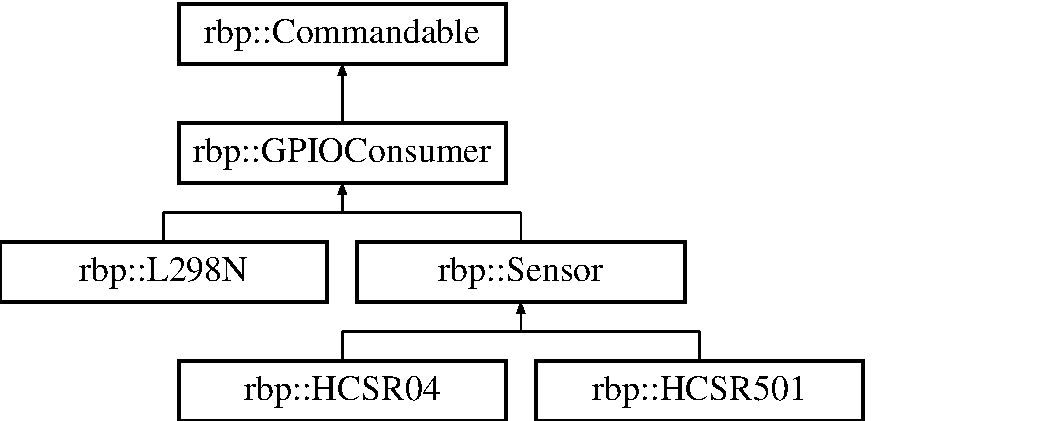
\includegraphics[height=4.000000cm]{classrbp_1_1Commandable}
\end{center}
\end{figure}
\subsection*{Public Member Functions}
\begin{DoxyCompactItemize}
\item 
virtual void \hyperlink{classrbp_1_1Commandable_a4a4214731d3e04b5590f805dd5f459f4}{Accept\+Command} (const \hyperlink{classrbp_1_1Command}{Command} \&data)=0
\begin{DoxyCompactList}\small\item\em Accepts a \hyperlink{classrbp_1_1Command}{Command} and performs an operation if the command exists within \hyperlink{classrbp_1_1Commandable_a8e6d397d308b8c075942bc1c8d6d7ca2}{Get\+Commands()} \end{DoxyCompactList}\item 
virtual std\+::map$<$ std\+::string, unsigned char $>$ \hyperlink{classrbp_1_1Commandable_a8e6d397d308b8c075942bc1c8d6d7ca2}{Get\+Commands} () const =0
\begin{DoxyCompactList}\small\item\em Get a map of a human readable string and its respective command I\+D. \end{DoxyCompactList}\item 
virtual const unsigned char \hyperlink{classrbp_1_1Commandable_a9f4e9e2b747133cdf1600f8bb82c4b02}{Get\+Component\+Id} () const =0
\begin{DoxyCompactList}\small\item\em Get the physical component\textquotesingle{}s I\+D. \end{DoxyCompactList}\item 
virtual void \hyperlink{classrbp_1_1Commandable_a19fb2e619697c9b9b77a638747cc4288}{Set\+Component\+Id} (unsigned char id)=0
\begin{DoxyCompactList}\small\item\em Set the physical component\textquotesingle{}s I\+D. \end{DoxyCompactList}\end{DoxyCompactItemize}


\subsection{Detailed Description}
Interface for objects that can accept Commands. 



\subsection{Member Function Documentation}
\hypertarget{classrbp_1_1Commandable_a4a4214731d3e04b5590f805dd5f459f4}{}\index{rbp\+::\+Commandable@{rbp\+::\+Commandable}!Accept\+Command@{Accept\+Command}}
\index{Accept\+Command@{Accept\+Command}!rbp\+::\+Commandable@{rbp\+::\+Commandable}}
\subsubsection[{Accept\+Command}]{\setlength{\rightskip}{0pt plus 5cm}virtual void rbp\+::\+Commandable\+::\+Accept\+Command (
\begin{DoxyParamCaption}
\item[{const {\bf Command} \&}]{data}
\end{DoxyParamCaption}
)\hspace{0.3cm}{\ttfamily [pure virtual]}}\label{classrbp_1_1Commandable_a4a4214731d3e04b5590f805dd5f459f4}


Accepts a \hyperlink{classrbp_1_1Command}{Command} and performs an operation if the command exists within \hyperlink{classrbp_1_1Commandable_a8e6d397d308b8c075942bc1c8d6d7ca2}{Get\+Commands()} 


\begin{DoxyParams}{Parameters}
{\em data} & The command to accept \\
\hline
\end{DoxyParams}


Implemented in \hyperlink{classrbp_1_1L298N_afa20e1274df6fb59a3d162e38b2408ea}{rbp\+::\+L298\+N}, \hyperlink{classrbp_1_1HCSR04_a5f7030ea092c72991fab902e1a2384f5}{rbp\+::\+H\+C\+S\+R04}, and \hyperlink{classrbp_1_1HCSR501_aac9cd8d47aa9df19fb04ed3972e89179}{rbp\+::\+H\+C\+S\+R501}.

\hypertarget{classrbp_1_1Commandable_a8e6d397d308b8c075942bc1c8d6d7ca2}{}\index{rbp\+::\+Commandable@{rbp\+::\+Commandable}!Get\+Commands@{Get\+Commands}}
\index{Get\+Commands@{Get\+Commands}!rbp\+::\+Commandable@{rbp\+::\+Commandable}}
\subsubsection[{Get\+Commands}]{\setlength{\rightskip}{0pt plus 5cm}virtual std\+::map$<$std\+::string, unsigned char$>$ rbp\+::\+Commandable\+::\+Get\+Commands (
\begin{DoxyParamCaption}
{}
\end{DoxyParamCaption}
) const\hspace{0.3cm}{\ttfamily [pure virtual]}}\label{classrbp_1_1Commandable_a8e6d397d308b8c075942bc1c8d6d7ca2}


Get a map of a human readable string and its respective command I\+D. 

\begin{DoxyReturn}{Returns}
A map of command names and respective I\+Ds 
\end{DoxyReturn}


Implemented in \hyperlink{classrbp_1_1L298N_ad3bae353e3d17675672286a68ced9d24}{rbp\+::\+L298\+N}, \hyperlink{classrbp_1_1HCSR04_ab418091c846e7256c6d937eb4cea60d0}{rbp\+::\+H\+C\+S\+R04}, and \hyperlink{classrbp_1_1HCSR501_a620a899944b11bf631e3616895fa5a77}{rbp\+::\+H\+C\+S\+R501}.

\hypertarget{classrbp_1_1Commandable_a9f4e9e2b747133cdf1600f8bb82c4b02}{}\index{rbp\+::\+Commandable@{rbp\+::\+Commandable}!Get\+Component\+Id@{Get\+Component\+Id}}
\index{Get\+Component\+Id@{Get\+Component\+Id}!rbp\+::\+Commandable@{rbp\+::\+Commandable}}
\subsubsection[{Get\+Component\+Id}]{\setlength{\rightskip}{0pt plus 5cm}virtual const unsigned char rbp\+::\+Commandable\+::\+Get\+Component\+Id (
\begin{DoxyParamCaption}
{}
\end{DoxyParamCaption}
) const\hspace{0.3cm}{\ttfamily [pure virtual]}}\label{classrbp_1_1Commandable_a9f4e9e2b747133cdf1600f8bb82c4b02}


Get the physical component\textquotesingle{}s I\+D. 

\begin{DoxyReturn}{Returns}
The physical component\textquotesingle{}s I\+D 
\end{DoxyReturn}


Implemented in \hyperlink{classrbp_1_1L298N_af4c1a48847326d4f962594cacbcdfa9c}{rbp\+::\+L298\+N}, \hyperlink{classrbp_1_1HCSR04_ac4bfc202a0d42469017bac7aedf03d77}{rbp\+::\+H\+C\+S\+R04}, and \hyperlink{classrbp_1_1HCSR501_a144ca65c1248656a016564493d59fe47}{rbp\+::\+H\+C\+S\+R501}.

\hypertarget{classrbp_1_1Commandable_a19fb2e619697c9b9b77a638747cc4288}{}\index{rbp\+::\+Commandable@{rbp\+::\+Commandable}!Set\+Component\+Id@{Set\+Component\+Id}}
\index{Set\+Component\+Id@{Set\+Component\+Id}!rbp\+::\+Commandable@{rbp\+::\+Commandable}}
\subsubsection[{Set\+Component\+Id}]{\setlength{\rightskip}{0pt plus 5cm}virtual void rbp\+::\+Commandable\+::\+Set\+Component\+Id (
\begin{DoxyParamCaption}
\item[{unsigned char}]{id}
\end{DoxyParamCaption}
)\hspace{0.3cm}{\ttfamily [pure virtual]}}\label{classrbp_1_1Commandable_a19fb2e619697c9b9b77a638747cc4288}


Set the physical component\textquotesingle{}s I\+D. 


\begin{DoxyParams}{Parameters}
{\em id} & The I\+D to use \\
\hline
\end{DoxyParams}


Implemented in \hyperlink{classrbp_1_1L298N_ae2557785a6795a727c6526baade4c174}{rbp\+::\+L298\+N}, \hyperlink{classrbp_1_1HCSR04_a32db67ffcb0adac730ed32523ceec111}{rbp\+::\+H\+C\+S\+R04}, and \hyperlink{classrbp_1_1HCSR501_a12e4d4dbdfce36157af3042fe65cbb50}{rbp\+::\+H\+C\+S\+R501}.



The documentation for this class was generated from the following file\+:\begin{DoxyCompactItemize}
\item 
include/raspboop/interfaces/Commandable.\+h\end{DoxyCompactItemize}

\hypertarget{classrbp_1_1GPIOConsumer}{}\section{rbp\+:\+:G\+P\+I\+O\+Consumer Class Reference}
\label{classrbp_1_1GPIOConsumer}\index{rbp\+::\+G\+P\+I\+O\+Consumer@{rbp\+::\+G\+P\+I\+O\+Consumer}}


Abstract class for all G\+P\+I\+O pin utilizers.  




{\ttfamily \#include $<$G\+P\+I\+O\+Consumer.\+h$>$}

Inheritance diagram for rbp\+:\+:G\+P\+I\+O\+Consumer\+:\begin{figure}[H]
\begin{center}
\leavevmode
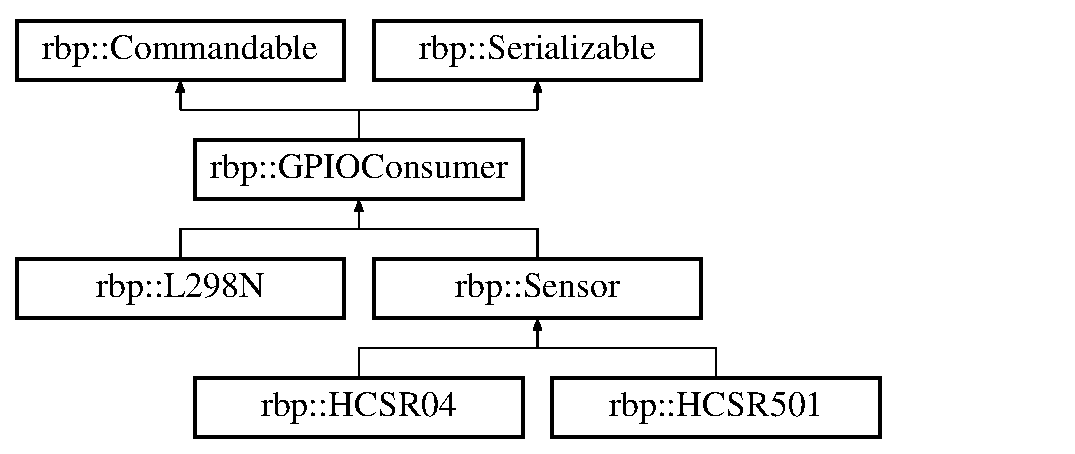
\includegraphics[height=4.000000cm]{classrbp_1_1GPIOConsumer}
\end{center}
\end{figure}
\subsection*{Public Member Functions}
\begin{DoxyCompactItemize}
\item 
\hypertarget{classrbp_1_1GPIOConsumer_a7cfe130a22c2c65526ba5fc8ff067786}{}std\+::vector$<$ int $>$ {\bfseries Get\+Pins} () const \label{classrbp_1_1GPIOConsumer_a7cfe130a22c2c65526ba5fc8ff067786}

\end{DoxyCompactItemize}
\subsection*{Protected Member Functions}
\begin{DoxyCompactItemize}
\item 
void \hyperlink{classrbp_1_1GPIOConsumer_ad705c79a02dcee7b0719ea2981d85866}{Consume\+Pin} (int pin, int mode)
\begin{DoxyCompactList}\small\item\em Reserves a pin and sets its mode. \end{DoxyCompactList}\end{DoxyCompactItemize}


\subsection{Detailed Description}
Abstract class for all G\+P\+I\+O pin utilizers. 

If a class will interface with the Raspberry Pi\textquotesingle{}s G\+P\+I\+O pins, then it must inherit from this class. This is to ensure that all children will be forced to use the {\ttfamily Release\+Pins()} method, which sets the value of any active pins to an inactive state.

Also, the {\ttfamily \hyperlink{classrbp_1_1GPIOConsumer_ad705c79a02dcee7b0719ea2981d85866}{Consume\+Pin()}} method provides a layer of abstraction over the wiring\+Pi {\ttfamily pin\+Mode()} method. In the future, this method will be a friend of the G\+P\+I\+O\+Manager class. 

\subsection{Member Function Documentation}
\hypertarget{classrbp_1_1GPIOConsumer_ad705c79a02dcee7b0719ea2981d85866}{}\index{rbp\+::\+G\+P\+I\+O\+Consumer@{rbp\+::\+G\+P\+I\+O\+Consumer}!Consume\+Pin@{Consume\+Pin}}
\index{Consume\+Pin@{Consume\+Pin}!rbp\+::\+G\+P\+I\+O\+Consumer@{rbp\+::\+G\+P\+I\+O\+Consumer}}
\subsubsection[{Consume\+Pin}]{\setlength{\rightskip}{0pt plus 5cm}void rbp\+::\+G\+P\+I\+O\+Consumer\+::\+Consume\+Pin (
\begin{DoxyParamCaption}
\item[{int}]{pin, }
\item[{int}]{mode}
\end{DoxyParamCaption}
)\hspace{0.3cm}{\ttfamily [protected]}}\label{classrbp_1_1GPIOConsumer_ad705c79a02dcee7b0719ea2981d85866}


Reserves a pin and sets its mode. 

Uses wiring\+Pi\textquotesingle{}s {\itshape pin\+Mode()} method to set the value of the {\itshape Pin} to the {\itshape Mode} parameter.


\begin{DoxyParams}{Parameters}
{\em Pin} & the G\+P\+I\+O pin to set \\
\hline
{\em Mode} & The Mode the Pin will be set to \\
\hline
\end{DoxyParams}


The documentation for this class was generated from the following files\+:\begin{DoxyCompactItemize}
\item 
include/raspboop/abstracts/G\+P\+I\+O\+Consumer.\+h\item 
src/abstracts/G\+P\+I\+O\+Consumer.\+cpp\end{DoxyCompactItemize}

\hypertarget{classrbp_1_1HCSR04}{}\section{rbp\+:\+:H\+C\+S\+R04 Class Reference}
\label{classrbp_1_1HCSR04}\index{rbp\+::\+H\+C\+S\+R04@{rbp\+::\+H\+C\+S\+R04}}


Ultrasonic distance sensor.  




{\ttfamily \#include $<$H\+C\+S\+R04.\+h$>$}

Inheritance diagram for rbp\+:\+:H\+C\+S\+R04\+:\begin{figure}[H]
\begin{center}
\leavevmode
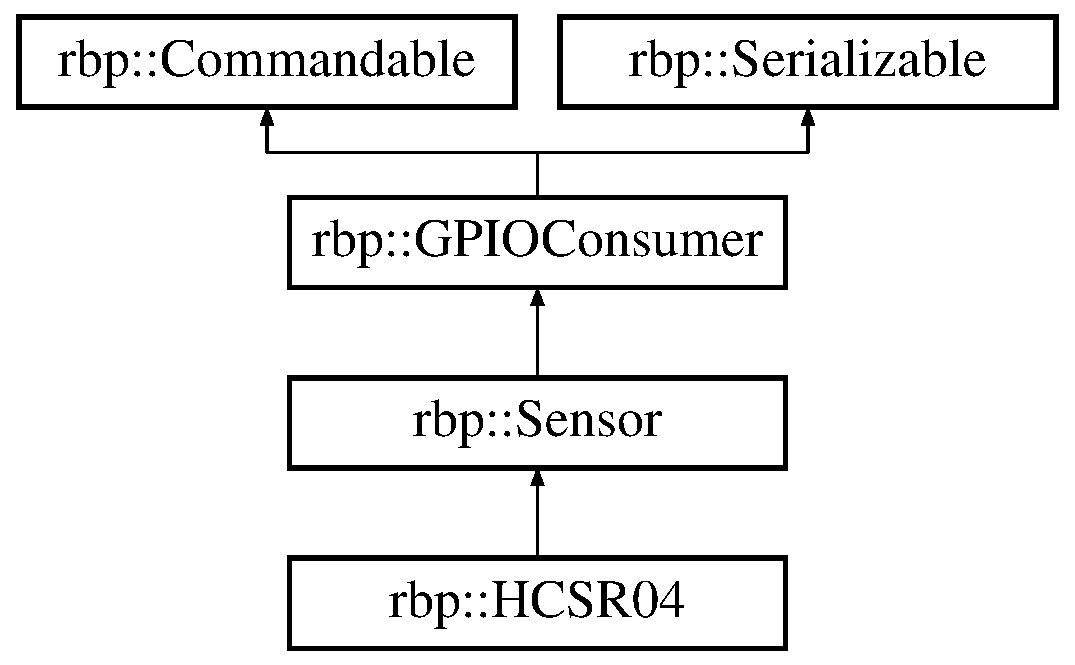
\includegraphics[height=4.000000cm]{classrbp_1_1HCSR04}
\end{center}
\end{figure}
\subsection*{Public Member Functions}
\begin{DoxyCompactItemize}
\item 
\hyperlink{classrbp_1_1HCSR04_aedc0e7fb482ff9c231693199acdef08a}{H\+C\+S\+R04} ()
\begin{DoxyCompactList}\small\item\em \hyperlink{classrbp_1_1HCSR04}{H\+C\+S\+R04} Constructor. \end{DoxyCompactList}\item 
virtual void \hyperlink{classrbp_1_1HCSR04_a8f8cc45655cacfb94ade5078c40ab1ba}{Sense} ()
\begin{DoxyCompactList}\small\item\em Performs the sensor\textquotesingle{}s sensing operation. \end{DoxyCompactList}\item 
float \hyperlink{classrbp_1_1HCSR04_aab17c63c05ffe5f351acc0112d6275cf}{Get\+Distance} () const 
\begin{DoxyCompactList}\small\item\em Get the distance calculated from the sensor. \end{DoxyCompactList}\item 
\hyperlink{classrbp_1_1HCSR04_a38f9bdcdff148fa58ee1c50661d9349f}{H\+C\+S\+R04} (int echo, int trig)
\begin{DoxyCompactList}\small\item\em Create a usable \hyperlink{classrbp_1_1HCSR04}{H\+C\+S\+R04} object. \end{DoxyCompactList}\item 
virtual void \hyperlink{classrbp_1_1HCSR04_a5f7030ea092c72991fab902e1a2384f5}{Accept\+Command} (const \hyperlink{classrbp_1_1Command}{Command} \&command)
\begin{DoxyCompactList}\small\item\em Accepts a \hyperlink{classrbp_1_1Command}{Command} and performs an operation if the command exists within \hyperlink{classrbp_1_1HCSR04_ab418091c846e7256c6d937eb4cea60d0}{Get\+Commands()} \end{DoxyCompactList}\item 
virtual std\+::map$<$ std\+::string, unsigned char $>$ \hyperlink{classrbp_1_1HCSR04_ab418091c846e7256c6d937eb4cea60d0}{Get\+Commands} () const 
\begin{DoxyCompactList}\small\item\em Get a map of a human readable string and its respective command I\+D. \end{DoxyCompactList}\item 
virtual const unsigned char \hyperlink{classrbp_1_1HCSR04_ac4bfc202a0d42469017bac7aedf03d77}{Get\+Component\+Id} () const 
\begin{DoxyCompactList}\small\item\em Get the physical component\textquotesingle{}s I\+D. \end{DoxyCompactList}\item 
virtual void \hyperlink{classrbp_1_1HCSR04_a32db67ffcb0adac730ed32523ceec111}{Set\+Component\+Id} (unsigned char id)
\begin{DoxyCompactList}\small\item\em Set the physical component\textquotesingle{}s I\+D. \end{DoxyCompactList}\item 
virtual std\+::vector$<$ unsigned char $>$ \hyperlink{classrbp_1_1HCSR04_aa4a535b88dfdf50a75a2374193038c32}{Serialize} ()
\begin{DoxyCompactList}\small\item\em Returns an array representation of an object. \end{DoxyCompactList}\item 
\hypertarget{classrbp_1_1HCSR04_ab5d6f623fccd8bb1dd782df8945a381d}{}\hyperlink{classrbp_1_1HCSR04_ab5d6f623fccd8bb1dd782df8945a381d}{$\sim$\+H\+C\+S\+R04} ()\label{classrbp_1_1HCSR04_ab5d6f623fccd8bb1dd782df8945a381d}

\begin{DoxyCompactList}\small\item\em \hyperlink{classrbp_1_1HCSR04}{H\+C\+S\+R04} Destructor. \end{DoxyCompactList}\end{DoxyCompactItemize}
\subsection*{Additional Inherited Members}


\subsection{Detailed Description}
Ultrasonic distance sensor. 

The \hyperlink{classrbp_1_1HCSR04}{H\+C\+S\+R04} is an ultrasonic distance sensor. By emitting an ultrasonic sound, the distance between the sensor and another object can be calculated through the formula\+:

d = t $\ast$ 340 /2

where, {\itshape d} is distance in meters, {\itshape t} is time in seconds, {\itshape 340} is the speed of sound in m/s

We divide by two because the sound had to travel back to the sensor.

\subsection*{Helpful information }


\begin{DoxyItemize}
\item The sensor has 4 pins
\begin{DoxyItemize}
\item {\bfseries Vcc} input 5\+V here
\item {\bfseries Trig} Input used to tell the sensor when to send the sound
\item {\bfseries Echo} The output from the sensor
\item {\bfseries G\+N\+D} Connect this to ground
\end{DoxyItemize}
\end{DoxyItemize}

{\bfseries I\+M\+P\+O\+R\+T\+A\+N\+T I\+N\+F\+O\+R\+M\+A\+T\+I\+O\+N\+:} The Raspberry Pi\textquotesingle{}s pins operate at 3\+V3 volt logic. This means that you must use a voltage divider on the Echo pin when reading in a value. I recommend using two resistors whose values are 1.\+5x apart. For more detailed instructions on how to do this, visit\+: \href{http://www.bytecreation.com/blog/2013/10/13/
 raspberry-pi-ultrasonic-sensor-hc-sr04}{\tt bytecreation.\+com}

\begin{TabularC}{2}
\hline
\rowcolor{lightgray}{\bf Quick Stats }&{\bf Value  }\\\cline{1-2}
Operating Voltage &{\bfseries 5\+V} \\\cline{1-2}
Operating Current &{\bfseries 15 m\+A} \\\cline{1-2}
Soundwave frequency &{\bfseries 40 Hz} \\\cline{1-2}
Maximum distance &{\bfseries 4m} \\\cline{1-2}
Minimum distance &{\bfseries 2 cm} \\\cline{1-2}
Required Trigger pulse &{\bfseries 10us (microseconds) H\+I\+G\+H signal} \\\cline{1-2}
\end{TabularC}


\subsubsection*{External links }

\href{http://users.ece.utexas.edu/~valvano/Datasheets/
HCSR04b.pdf}{\tt Datasheet}

\href{http://www.bytecreation.com/blog/2013/10/13/
raspberry-pi-ultrasonic-sensor-hc-sr04}{\tt Blog post\+:} Good article that details the steps necessary to use this sensor with a raspberry pi and a voltage divider. 

\subsection{Constructor \& Destructor Documentation}
\hypertarget{classrbp_1_1HCSR04_aedc0e7fb482ff9c231693199acdef08a}{}\index{rbp\+::\+H\+C\+S\+R04@{rbp\+::\+H\+C\+S\+R04}!H\+C\+S\+R04@{H\+C\+S\+R04}}
\index{H\+C\+S\+R04@{H\+C\+S\+R04}!rbp\+::\+H\+C\+S\+R04@{rbp\+::\+H\+C\+S\+R04}}
\subsubsection[{H\+C\+S\+R04}]{\setlength{\rightskip}{0pt plus 5cm}rbp\+::\+H\+C\+S\+R04\+::\+H\+C\+S\+R04 (
\begin{DoxyParamCaption}
{}
\end{DoxyParamCaption}
)}\label{classrbp_1_1HCSR04_aedc0e7fb482ff9c231693199acdef08a}


\hyperlink{classrbp_1_1HCSR04}{H\+C\+S\+R04} Constructor. 

Initializes all private member variables to unused values. \hypertarget{classrbp_1_1HCSR04_a38f9bdcdff148fa58ee1c50661d9349f}{}\index{rbp\+::\+H\+C\+S\+R04@{rbp\+::\+H\+C\+S\+R04}!H\+C\+S\+R04@{H\+C\+S\+R04}}
\index{H\+C\+S\+R04@{H\+C\+S\+R04}!rbp\+::\+H\+C\+S\+R04@{rbp\+::\+H\+C\+S\+R04}}
\subsubsection[{H\+C\+S\+R04}]{\setlength{\rightskip}{0pt plus 5cm}rbp\+::\+H\+C\+S\+R04\+::\+H\+C\+S\+R04 (
\begin{DoxyParamCaption}
\item[{int}]{echo, }
\item[{int}]{trig}
\end{DoxyParamCaption}
)}\label{classrbp_1_1HCSR04_a38f9bdcdff148fa58ee1c50661d9349f}


Create a usable \hyperlink{classrbp_1_1HCSR04}{H\+C\+S\+R04} object. 

Initializes the \hyperlink{classrbp_1_1HCSR04}{H\+C\+S\+R04}\textquotesingle{}s pins using the \hyperlink{classrbp_1_1Sensor_a2e3a00de93b77ecf39b4bfee79279c3c}{Set\+Input\+Pin()} and \hyperlink{classrbp_1_1Sensor_aab6baaef855fd31dab94e5b28386410a}{Set\+Output\+Pin()} methods inherited from \hyperlink{classrbp_1_1Sensor}{Sensor}.


\begin{DoxyParams}{Parameters}
{\em echo} & The input pin designated to read the sensors E\+C\+H\+O output \\
\hline
{\em trig} & The output pin that initiates sensing \\
\hline
\end{DoxyParams}


\subsection{Member Function Documentation}
\hypertarget{classrbp_1_1HCSR04_a5f7030ea092c72991fab902e1a2384f5}{}\index{rbp\+::\+H\+C\+S\+R04@{rbp\+::\+H\+C\+S\+R04}!Accept\+Command@{Accept\+Command}}
\index{Accept\+Command@{Accept\+Command}!rbp\+::\+H\+C\+S\+R04@{rbp\+::\+H\+C\+S\+R04}}
\subsubsection[{Accept\+Command}]{\setlength{\rightskip}{0pt plus 5cm}void rbp\+::\+H\+C\+S\+R04\+::\+Accept\+Command (
\begin{DoxyParamCaption}
\item[{const {\bf Command} \&}]{data}
\end{DoxyParamCaption}
)\hspace{0.3cm}{\ttfamily [virtual]}}\label{classrbp_1_1HCSR04_a5f7030ea092c72991fab902e1a2384f5}


Accepts a \hyperlink{classrbp_1_1Command}{Command} and performs an operation if the command exists within \hyperlink{classrbp_1_1HCSR04_ab418091c846e7256c6d937eb4cea60d0}{Get\+Commands()} 


\begin{DoxyParams}{Parameters}
{\em data} & The command to accept \\
\hline
\end{DoxyParams}


Implements \hyperlink{classrbp_1_1Commandable_a4a4214731d3e04b5590f805dd5f459f4}{rbp\+::\+Commandable}.

\hypertarget{classrbp_1_1HCSR04_ab418091c846e7256c6d937eb4cea60d0}{}\index{rbp\+::\+H\+C\+S\+R04@{rbp\+::\+H\+C\+S\+R04}!Get\+Commands@{Get\+Commands}}
\index{Get\+Commands@{Get\+Commands}!rbp\+::\+H\+C\+S\+R04@{rbp\+::\+H\+C\+S\+R04}}
\subsubsection[{Get\+Commands}]{\setlength{\rightskip}{0pt plus 5cm}std\+::map$<$ std\+::string, unsigned char $>$ rbp\+::\+H\+C\+S\+R04\+::\+Get\+Commands (
\begin{DoxyParamCaption}
{}
\end{DoxyParamCaption}
) const\hspace{0.3cm}{\ttfamily [virtual]}}\label{classrbp_1_1HCSR04_ab418091c846e7256c6d937eb4cea60d0}


Get a map of a human readable string and its respective command I\+D. 

\begin{DoxyReturn}{Returns}
A map of command names and respective I\+Ds 
\end{DoxyReturn}


Implements \hyperlink{classrbp_1_1Commandable_a8e6d397d308b8c075942bc1c8d6d7ca2}{rbp\+::\+Commandable}.

\hypertarget{classrbp_1_1HCSR04_ac4bfc202a0d42469017bac7aedf03d77}{}\index{rbp\+::\+H\+C\+S\+R04@{rbp\+::\+H\+C\+S\+R04}!Get\+Component\+Id@{Get\+Component\+Id}}
\index{Get\+Component\+Id@{Get\+Component\+Id}!rbp\+::\+H\+C\+S\+R04@{rbp\+::\+H\+C\+S\+R04}}
\subsubsection[{Get\+Component\+Id}]{\setlength{\rightskip}{0pt plus 5cm}const unsigned char rbp\+::\+H\+C\+S\+R04\+::\+Get\+Component\+Id (
\begin{DoxyParamCaption}
{}
\end{DoxyParamCaption}
) const\hspace{0.3cm}{\ttfamily [virtual]}}\label{classrbp_1_1HCSR04_ac4bfc202a0d42469017bac7aedf03d77}


Get the physical component\textquotesingle{}s I\+D. 

\begin{DoxyReturn}{Returns}
The physical component\textquotesingle{}s I\+D 
\end{DoxyReturn}


Implements \hyperlink{classrbp_1_1Commandable_a9f4e9e2b747133cdf1600f8bb82c4b02}{rbp\+::\+Commandable}.

\hypertarget{classrbp_1_1HCSR04_aab17c63c05ffe5f351acc0112d6275cf}{}\index{rbp\+::\+H\+C\+S\+R04@{rbp\+::\+H\+C\+S\+R04}!Get\+Distance@{Get\+Distance}}
\index{Get\+Distance@{Get\+Distance}!rbp\+::\+H\+C\+S\+R04@{rbp\+::\+H\+C\+S\+R04}}
\subsubsection[{Get\+Distance}]{\setlength{\rightskip}{0pt plus 5cm}float rbp\+::\+H\+C\+S\+R04\+::\+Get\+Distance (
\begin{DoxyParamCaption}
{}
\end{DoxyParamCaption}
) const\hspace{0.3cm}{\ttfamily [inline]}}\label{classrbp_1_1HCSR04_aab17c63c05ffe5f351acc0112d6275cf}


Get the distance calculated from the sensor. 

\begin{DoxyReturn}{Returns}
A float representing the distance sensed in centimeters 
\end{DoxyReturn}
\hypertarget{classrbp_1_1HCSR04_a8f8cc45655cacfb94ade5078c40ab1ba}{}\index{rbp\+::\+H\+C\+S\+R04@{rbp\+::\+H\+C\+S\+R04}!Sense@{Sense}}
\index{Sense@{Sense}!rbp\+::\+H\+C\+S\+R04@{rbp\+::\+H\+C\+S\+R04}}
\subsubsection[{Sense}]{\setlength{\rightskip}{0pt plus 5cm}void rbp\+::\+H\+C\+S\+R04\+::\+Sense (
\begin{DoxyParamCaption}
{}
\end{DoxyParamCaption}
)\hspace{0.3cm}{\ttfamily [virtual]}}\label{classrbp_1_1HCSR04_a8f8cc45655cacfb94ade5078c40ab1ba}


Performs the sensor\textquotesingle{}s sensing operation. 

This method will retrieve a value from the environment by performing G\+P\+I\+O operations on the input and output pins of the sensor. The value from the sensor will be available through an accessor method. 

Implements \hyperlink{classrbp_1_1Sensor_ab9d45316bf67d871fddc7aa048e89c49}{rbp\+::\+Sensor}.

\hypertarget{classrbp_1_1HCSR04_aa4a535b88dfdf50a75a2374193038c32}{}\index{rbp\+::\+H\+C\+S\+R04@{rbp\+::\+H\+C\+S\+R04}!Serialize@{Serialize}}
\index{Serialize@{Serialize}!rbp\+::\+H\+C\+S\+R04@{rbp\+::\+H\+C\+S\+R04}}
\subsubsection[{Serialize}]{\setlength{\rightskip}{0pt plus 5cm}std\+::vector$<$ unsigned char $>$ rbp\+::\+H\+C\+S\+R04\+::\+Serialize (
\begin{DoxyParamCaption}
{}
\end{DoxyParamCaption}
)\hspace{0.3cm}{\ttfamily [virtual]}}\label{classrbp_1_1HCSR04_aa4a535b88dfdf50a75a2374193038c32}


Returns an array representation of an object. 

\begin{DoxyReturn}{Returns}
The Buffer of data 
\end{DoxyReturn}


Implements \hyperlink{classrbp_1_1Serializable_a349896f5c3356330f914621033fda0bb}{rbp\+::\+Serializable}.

\hypertarget{classrbp_1_1HCSR04_a32db67ffcb0adac730ed32523ceec111}{}\index{rbp\+::\+H\+C\+S\+R04@{rbp\+::\+H\+C\+S\+R04}!Set\+Component\+Id@{Set\+Component\+Id}}
\index{Set\+Component\+Id@{Set\+Component\+Id}!rbp\+::\+H\+C\+S\+R04@{rbp\+::\+H\+C\+S\+R04}}
\subsubsection[{Set\+Component\+Id}]{\setlength{\rightskip}{0pt plus 5cm}void rbp\+::\+H\+C\+S\+R04\+::\+Set\+Component\+Id (
\begin{DoxyParamCaption}
\item[{unsigned char}]{id}
\end{DoxyParamCaption}
)\hspace{0.3cm}{\ttfamily [virtual]}}\label{classrbp_1_1HCSR04_a32db67ffcb0adac730ed32523ceec111}


Set the physical component\textquotesingle{}s I\+D. 


\begin{DoxyParams}{Parameters}
{\em id} & The I\+D to use \\
\hline
\end{DoxyParams}


Implements \hyperlink{classrbp_1_1Commandable_a19fb2e619697c9b9b77a638747cc4288}{rbp\+::\+Commandable}.



The documentation for this class was generated from the following files\+:\begin{DoxyCompactItemize}
\item 
include/raspboop/sensors/H\+C\+S\+R04.\+h\item 
src/sensors/H\+C\+S\+R04.\+cpp\end{DoxyCompactItemize}

\hypertarget{classrbp_1_1HCSR501}{}\section{rbp\+:\+:H\+C\+S\+R501 Class Reference}
\label{classrbp_1_1HCSR501}\index{rbp\+::\+H\+C\+S\+R501@{rbp\+::\+H\+C\+S\+R501}}


Passive infrared sensor for motion detection.  




{\ttfamily \#include $<$H\+C\+S\+R501.\+h$>$}

Inheritance diagram for rbp\+:\+:H\+C\+S\+R501\+:\begin{figure}[H]
\begin{center}
\leavevmode
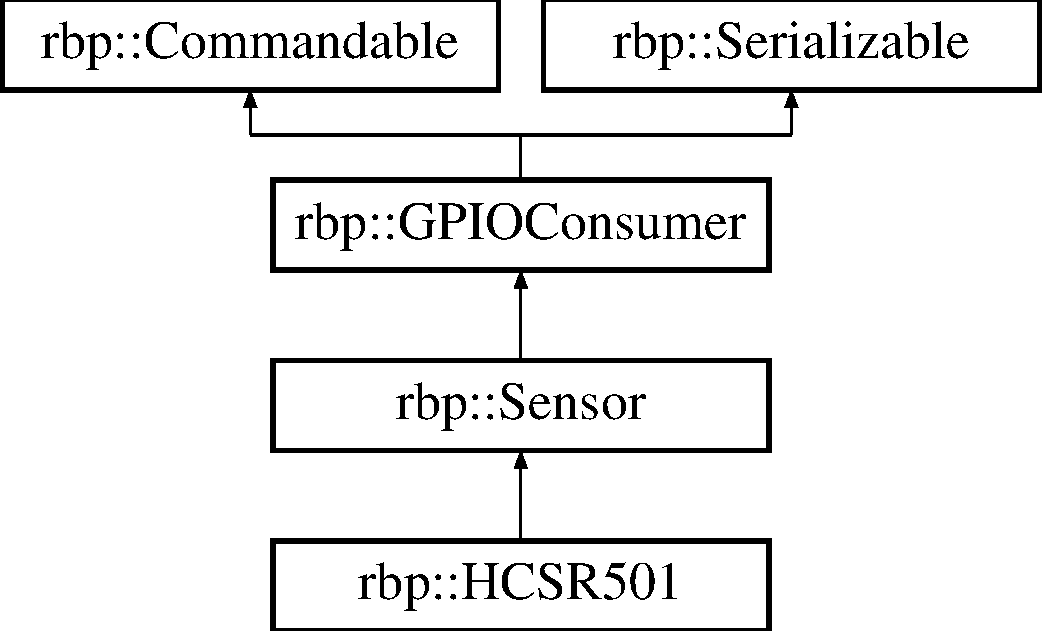
\includegraphics[height=4.000000cm]{classrbp_1_1HCSR501}
\end{center}
\end{figure}
\subsection*{Public Member Functions}
\begin{DoxyCompactItemize}
\item 
\hyperlink{classrbp_1_1HCSR501_ae6fa939683256d390886b07ef2b2861e}{H\+C\+S\+R501} ()
\begin{DoxyCompactList}\small\item\em \hyperlink{classrbp_1_1HCSR501}{H\+C\+S\+R501} Constructor. \end{DoxyCompactList}\item 
\hyperlink{classrbp_1_1HCSR501_a061fd4c0a4e51ad6118add781b523cbb}{H\+C\+S\+R501} (int signal)
\begin{DoxyCompactList}\small\item\em Create a usable \hyperlink{classrbp_1_1HCSR501}{H\+C\+S\+R501} object. \end{DoxyCompactList}\item 
virtual void \hyperlink{classrbp_1_1HCSR501_a9b0e9b6f210d269b67a1ec94e3b62359}{Sense} ()
\begin{DoxyCompactList}\small\item\em Performs the sensor\textquotesingle{}s sensing operation. \end{DoxyCompactList}\item 
bool \hyperlink{classrbp_1_1HCSR501_a61d40d80c544ffaf3ab75adcd03fdcb3}{Is\+Signalled} () const 
\begin{DoxyCompactList}\small\item\em Get the value obtained from \hyperlink{classrbp_1_1HCSR501_a9b0e9b6f210d269b67a1ec94e3b62359}{Sense()} \end{DoxyCompactList}\item 
virtual void \hyperlink{classrbp_1_1HCSR501_aac9cd8d47aa9df19fb04ed3972e89179}{Accept\+Command} (const \hyperlink{classrbp_1_1Command}{Command} \&command)
\begin{DoxyCompactList}\small\item\em Accepts a \hyperlink{classrbp_1_1Command}{Command} and performs an operation if the command exists within \hyperlink{classrbp_1_1HCSR501_a620a899944b11bf631e3616895fa5a77}{Get\+Commands()} \end{DoxyCompactList}\item 
virtual std\+::map$<$ std\+::string, unsigned char $>$ \hyperlink{classrbp_1_1HCSR501_a620a899944b11bf631e3616895fa5a77}{Get\+Commands} () const 
\begin{DoxyCompactList}\small\item\em Get a map of a human readable string and its respective command I\+D. \end{DoxyCompactList}\item 
virtual const unsigned char \hyperlink{classrbp_1_1HCSR501_a144ca65c1248656a016564493d59fe47}{Get\+Component\+Id} () const 
\begin{DoxyCompactList}\small\item\em Get the physical component\textquotesingle{}s I\+D. \end{DoxyCompactList}\item 
virtual void \hyperlink{classrbp_1_1HCSR501_a12e4d4dbdfce36157af3042fe65cbb50}{Set\+Component\+Id} (unsigned char id)
\begin{DoxyCompactList}\small\item\em Set the physical component\textquotesingle{}s I\+D. \end{DoxyCompactList}\item 
virtual std\+::vector$<$ unsigned char $>$ \hyperlink{classrbp_1_1HCSR501_a6aa46721ed0dcba774435a24ac17072e}{Serialize} ()
\begin{DoxyCompactList}\small\item\em Returns an array representation of an object. \end{DoxyCompactList}\item 
\hypertarget{classrbp_1_1HCSR501_a9ba22950944715359016ed2f81e5a9ea}{}\hyperlink{classrbp_1_1HCSR501_a9ba22950944715359016ed2f81e5a9ea}{$\sim$\+H\+C\+S\+R501} ()\label{classrbp_1_1HCSR501_a9ba22950944715359016ed2f81e5a9ea}

\begin{DoxyCompactList}\small\item\em \hyperlink{classrbp_1_1HCSR501}{H\+C\+S\+R501} destructor. \end{DoxyCompactList}\end{DoxyCompactItemize}
\subsection*{Additional Inherited Members}


\subsection{Detailed Description}
Passive infrared sensor for motion detection. 

The \hyperlink{classrbp_1_1HCSR501}{H\+C\+S\+R501} is a passive infrared sensor used for motion detection applications. There are 5 main pins that you will need to be familiar with\+:


\begin{DoxyItemize}
\item 5\+V input
\item Signal
\item Gnd
\item retriggering pin
\item non-\/retriggering pin
\end{DoxyItemize}

\subsection*{Helpful information }

There are two modes to the sensor\+: retriggering, and non-\/retriggering. In retriggering mode, signal outputs high as long as motion is detected. In non-\/retriggering mode, signal will output as H\+I\+G\+H only every second or so that motion is detected.

\begin{TabularC}{2}
\hline
\rowcolor{lightgray}{\bf Quick Stats }&{\bf Value  }\\\cline{1-2}
Vcc &{\bfseries 5-\/16\+V} \\\cline{1-2}
Logical voltage &{\bfseries 3\+V3} \\\cline{1-2}
Sensing range &{\bfseries 7 meters} \\\cline{1-2}
\end{TabularC}
\subsubsection*{External Links }

\href{http://www.ladyada.net/media/
sensors/PIRSensor-V1.2.pdf}{\tt Parallax P\+I\+R datasheet}

\href{http://elecfreaks.com/store/download/
datasheet/sensor/DYP-ME003/Specification.pdf}{\tt Elec Freaks datasheet}

\href{http://
www.ladyada.net/learn/sensors/pir.html}{\tt P\+I\+R motion sensors tutorial by Lady\+Ada.\+net}

\href{http://robotic-controls.com/learn/sensors/pir-sensor-hc-sr501}{\tt Supplementary Arduino code and tutorial} 

\subsection{Constructor \& Destructor Documentation}
\hypertarget{classrbp_1_1HCSR501_ae6fa939683256d390886b07ef2b2861e}{}\index{rbp\+::\+H\+C\+S\+R501@{rbp\+::\+H\+C\+S\+R501}!H\+C\+S\+R501@{H\+C\+S\+R501}}
\index{H\+C\+S\+R501@{H\+C\+S\+R501}!rbp\+::\+H\+C\+S\+R501@{rbp\+::\+H\+C\+S\+R501}}
\subsubsection[{H\+C\+S\+R501}]{\setlength{\rightskip}{0pt plus 5cm}rbp\+::\+H\+C\+S\+R501\+::\+H\+C\+S\+R501 (
\begin{DoxyParamCaption}
{}
\end{DoxyParamCaption}
)}\label{classrbp_1_1HCSR501_ae6fa939683256d390886b07ef2b2861e}


\hyperlink{classrbp_1_1HCSR501}{H\+C\+S\+R501} Constructor. 

Initializes private variables to unused values \hypertarget{classrbp_1_1HCSR501_a061fd4c0a4e51ad6118add781b523cbb}{}\index{rbp\+::\+H\+C\+S\+R501@{rbp\+::\+H\+C\+S\+R501}!H\+C\+S\+R501@{H\+C\+S\+R501}}
\index{H\+C\+S\+R501@{H\+C\+S\+R501}!rbp\+::\+H\+C\+S\+R501@{rbp\+::\+H\+C\+S\+R501}}
\subsubsection[{H\+C\+S\+R501}]{\setlength{\rightskip}{0pt plus 5cm}rbp\+::\+H\+C\+S\+R501\+::\+H\+C\+S\+R501 (
\begin{DoxyParamCaption}
\item[{int}]{signal}
\end{DoxyParamCaption}
)}\label{classrbp_1_1HCSR501_a061fd4c0a4e51ad6118add781b523cbb}


Create a usable \hyperlink{classrbp_1_1HCSR501}{H\+C\+S\+R501} object. 

Initializes the \hyperlink{classrbp_1_1HCSR501}{H\+C\+S\+R501}\textquotesingle{}s Signal pin using the \hyperlink{classrbp_1_1Sensor_a2e3a00de93b77ecf39b4bfee79279c3c}{Set\+Input\+Pin()} method from \hyperlink{classrbp_1_1Sensor}{Sensor}.


\begin{DoxyParams}{Parameters}
{\em signal} & The input pin which will read the value from the sensor \\
\hline
\end{DoxyParams}


\subsection{Member Function Documentation}
\hypertarget{classrbp_1_1HCSR501_aac9cd8d47aa9df19fb04ed3972e89179}{}\index{rbp\+::\+H\+C\+S\+R501@{rbp\+::\+H\+C\+S\+R501}!Accept\+Command@{Accept\+Command}}
\index{Accept\+Command@{Accept\+Command}!rbp\+::\+H\+C\+S\+R501@{rbp\+::\+H\+C\+S\+R501}}
\subsubsection[{Accept\+Command}]{\setlength{\rightskip}{0pt plus 5cm}void rbp\+::\+H\+C\+S\+R501\+::\+Accept\+Command (
\begin{DoxyParamCaption}
\item[{const {\bf Command} \&}]{data}
\end{DoxyParamCaption}
)\hspace{0.3cm}{\ttfamily [virtual]}}\label{classrbp_1_1HCSR501_aac9cd8d47aa9df19fb04ed3972e89179}


Accepts a \hyperlink{classrbp_1_1Command}{Command} and performs an operation if the command exists within \hyperlink{classrbp_1_1HCSR501_a620a899944b11bf631e3616895fa5a77}{Get\+Commands()} 


\begin{DoxyParams}{Parameters}
{\em data} & The command to accept \\
\hline
\end{DoxyParams}


Implements \hyperlink{classrbp_1_1Commandable_a4a4214731d3e04b5590f805dd5f459f4}{rbp\+::\+Commandable}.

\hypertarget{classrbp_1_1HCSR501_a620a899944b11bf631e3616895fa5a77}{}\index{rbp\+::\+H\+C\+S\+R501@{rbp\+::\+H\+C\+S\+R501}!Get\+Commands@{Get\+Commands}}
\index{Get\+Commands@{Get\+Commands}!rbp\+::\+H\+C\+S\+R501@{rbp\+::\+H\+C\+S\+R501}}
\subsubsection[{Get\+Commands}]{\setlength{\rightskip}{0pt plus 5cm}std\+::map$<$ std\+::string, unsigned char $>$ rbp\+::\+H\+C\+S\+R501\+::\+Get\+Commands (
\begin{DoxyParamCaption}
{}
\end{DoxyParamCaption}
) const\hspace{0.3cm}{\ttfamily [virtual]}}\label{classrbp_1_1HCSR501_a620a899944b11bf631e3616895fa5a77}


Get a map of a human readable string and its respective command I\+D. 

\begin{DoxyReturn}{Returns}
A map of command names and respective I\+Ds 
\end{DoxyReturn}


Implements \hyperlink{classrbp_1_1Commandable_a8e6d397d308b8c075942bc1c8d6d7ca2}{rbp\+::\+Commandable}.

\hypertarget{classrbp_1_1HCSR501_a144ca65c1248656a016564493d59fe47}{}\index{rbp\+::\+H\+C\+S\+R501@{rbp\+::\+H\+C\+S\+R501}!Get\+Component\+Id@{Get\+Component\+Id}}
\index{Get\+Component\+Id@{Get\+Component\+Id}!rbp\+::\+H\+C\+S\+R501@{rbp\+::\+H\+C\+S\+R501}}
\subsubsection[{Get\+Component\+Id}]{\setlength{\rightskip}{0pt plus 5cm}const unsigned char rbp\+::\+H\+C\+S\+R501\+::\+Get\+Component\+Id (
\begin{DoxyParamCaption}
{}
\end{DoxyParamCaption}
) const\hspace{0.3cm}{\ttfamily [virtual]}}\label{classrbp_1_1HCSR501_a144ca65c1248656a016564493d59fe47}


Get the physical component\textquotesingle{}s I\+D. 

\begin{DoxyReturn}{Returns}
The physical component\textquotesingle{}s I\+D 
\end{DoxyReturn}


Implements \hyperlink{classrbp_1_1Commandable_a9f4e9e2b747133cdf1600f8bb82c4b02}{rbp\+::\+Commandable}.

\hypertarget{classrbp_1_1HCSR501_a61d40d80c544ffaf3ab75adcd03fdcb3}{}\index{rbp\+::\+H\+C\+S\+R501@{rbp\+::\+H\+C\+S\+R501}!Is\+Signalled@{Is\+Signalled}}
\index{Is\+Signalled@{Is\+Signalled}!rbp\+::\+H\+C\+S\+R501@{rbp\+::\+H\+C\+S\+R501}}
\subsubsection[{Is\+Signalled}]{\setlength{\rightskip}{0pt plus 5cm}bool rbp\+::\+H\+C\+S\+R501\+::\+Is\+Signalled (
\begin{DoxyParamCaption}
{}
\end{DoxyParamCaption}
) const\hspace{0.3cm}{\ttfamily [inline]}}\label{classrbp_1_1HCSR501_a61d40d80c544ffaf3ab75adcd03fdcb3}


Get the value obtained from \hyperlink{classrbp_1_1HCSR501_a9b0e9b6f210d269b67a1ec94e3b62359}{Sense()} 

\begin{DoxyReturn}{Returns}
A boolean value determining the signal pin\textquotesingle{}s value 
\end{DoxyReturn}
\hypertarget{classrbp_1_1HCSR501_a9b0e9b6f210d269b67a1ec94e3b62359}{}\index{rbp\+::\+H\+C\+S\+R501@{rbp\+::\+H\+C\+S\+R501}!Sense@{Sense}}
\index{Sense@{Sense}!rbp\+::\+H\+C\+S\+R501@{rbp\+::\+H\+C\+S\+R501}}
\subsubsection[{Sense}]{\setlength{\rightskip}{0pt plus 5cm}void rbp\+::\+H\+C\+S\+R501\+::\+Sense (
\begin{DoxyParamCaption}
{}
\end{DoxyParamCaption}
)\hspace{0.3cm}{\ttfamily [virtual]}}\label{classrbp_1_1HCSR501_a9b0e9b6f210d269b67a1ec94e3b62359}


Performs the sensor\textquotesingle{}s sensing operation. 

This method will retrieve a value from the environment by performing G\+P\+I\+O operations on the input and output pins of the sensor. The value from the sensor will be available through an accessor method. 

Implements \hyperlink{classrbp_1_1Sensor_ab9d45316bf67d871fddc7aa048e89c49}{rbp\+::\+Sensor}.

\hypertarget{classrbp_1_1HCSR501_a6aa46721ed0dcba774435a24ac17072e}{}\index{rbp\+::\+H\+C\+S\+R501@{rbp\+::\+H\+C\+S\+R501}!Serialize@{Serialize}}
\index{Serialize@{Serialize}!rbp\+::\+H\+C\+S\+R501@{rbp\+::\+H\+C\+S\+R501}}
\subsubsection[{Serialize}]{\setlength{\rightskip}{0pt plus 5cm}std\+::vector$<$ unsigned char $>$ rbp\+::\+H\+C\+S\+R501\+::\+Serialize (
\begin{DoxyParamCaption}
{}
\end{DoxyParamCaption}
)\hspace{0.3cm}{\ttfamily [virtual]}}\label{classrbp_1_1HCSR501_a6aa46721ed0dcba774435a24ac17072e}


Returns an array representation of an object. 

\begin{DoxyReturn}{Returns}
The Buffer of data 
\end{DoxyReturn}


Implements \hyperlink{classrbp_1_1Serializable_a349896f5c3356330f914621033fda0bb}{rbp\+::\+Serializable}.

\hypertarget{classrbp_1_1HCSR501_a12e4d4dbdfce36157af3042fe65cbb50}{}\index{rbp\+::\+H\+C\+S\+R501@{rbp\+::\+H\+C\+S\+R501}!Set\+Component\+Id@{Set\+Component\+Id}}
\index{Set\+Component\+Id@{Set\+Component\+Id}!rbp\+::\+H\+C\+S\+R501@{rbp\+::\+H\+C\+S\+R501}}
\subsubsection[{Set\+Component\+Id}]{\setlength{\rightskip}{0pt plus 5cm}void rbp\+::\+H\+C\+S\+R501\+::\+Set\+Component\+Id (
\begin{DoxyParamCaption}
\item[{unsigned char}]{id}
\end{DoxyParamCaption}
)\hspace{0.3cm}{\ttfamily [virtual]}}\label{classrbp_1_1HCSR501_a12e4d4dbdfce36157af3042fe65cbb50}


Set the physical component\textquotesingle{}s I\+D. 


\begin{DoxyParams}{Parameters}
{\em id} & The I\+D to use \\
\hline
\end{DoxyParams}


Implements \hyperlink{classrbp_1_1Commandable_a19fb2e619697c9b9b77a638747cc4288}{rbp\+::\+Commandable}.



The documentation for this class was generated from the following files\+:\begin{DoxyCompactItemize}
\item 
include/raspboop/sensors/H\+C\+S\+R501.\+h\item 
src/sensors/H\+C\+S\+R501.\+cpp\end{DoxyCompactItemize}

\hypertarget{classrbp_1_1L298N}{}\section{rbp\+:\+:L298\+N Class Reference}
\label{classrbp_1_1L298N}\index{rbp\+::\+L298\+N@{rbp\+::\+L298\+N}}


\hyperlink{classrbp_1_1L298N}{L298\+N} Motor controller.  




{\ttfamily \#include $<$L298\+N.\+h$>$}

Inheritance diagram for rbp\+:\+:L298\+N\+:\begin{figure}[H]
\begin{center}
\leavevmode
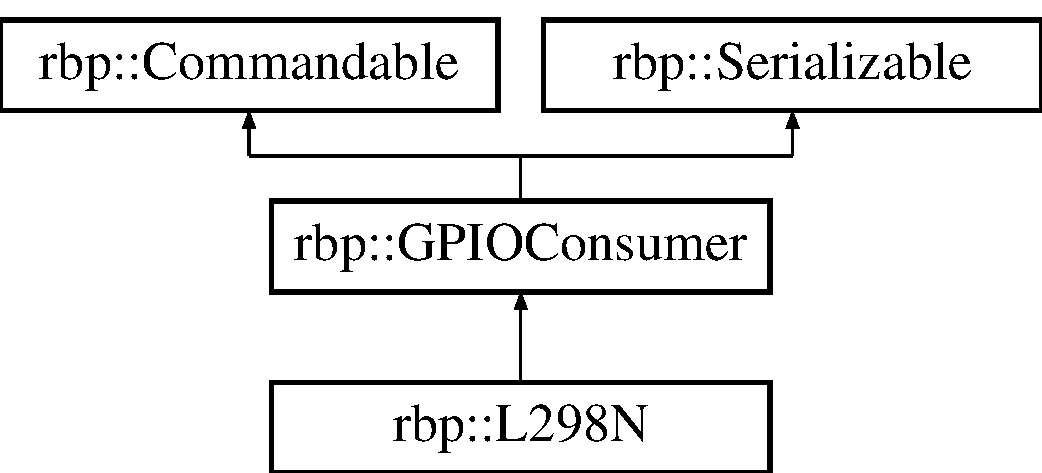
\includegraphics[height=3.000000cm]{classrbp_1_1L298N}
\end{center}
\end{figure}
\subsection*{Public Member Functions}
\begin{DoxyCompactItemize}
\item 
\hyperlink{classrbp_1_1L298N_aa825d425be63819ee0ec35fac3fcdecf}{L298\+N} (int in1, int in2, int in3, int in4)
\begin{DoxyCompactList}\small\item\em Creates an \hyperlink{classrbp_1_1L298N}{L298\+N} object. \end{DoxyCompactList}\item 
void \hyperlink{classrbp_1_1L298N_ac618a203bef8bb8afbe194740be501a5}{Use\+Soft\+P\+W\+M} ()
\begin{DoxyCompactList}\small\item\em Sets the input pins to software P\+W\+M mode. \end{DoxyCompactList}\item 
void \hyperlink{classrbp_1_1L298N_a5fcc1b9a3c9f2812e8adefb49cb704ef}{Set\+P\+W\+M\+Value} (int in, int value)
\begin{DoxyCompactList}\small\item\em Sets a pin\textquotesingle{}s software P\+W\+M value. \end{DoxyCompactList}\item 
void \hyperlink{classrbp_1_1L298N_a65f4f98d23ddae3d659ce3f5084cbd1e}{Set\+Pin\+Value} (int in, int value)
\begin{DoxyCompactList}\small\item\em Set a pin\textquotesingle{}s value to either H\+I\+G\+H or L\+O\+W. \end{DoxyCompactList}\item 
virtual void \hyperlink{classrbp_1_1L298N_afa20e1274df6fb59a3d162e38b2408ea}{Accept\+Command} (const \hyperlink{classrbp_1_1Command}{Command} \&command)
\begin{DoxyCompactList}\small\item\em Accepts a \hyperlink{classrbp_1_1Command}{Command} and performs an operation if the command exists within \hyperlink{classrbp_1_1L298N_ad3bae353e3d17675672286a68ced9d24}{Get\+Commands()} \end{DoxyCompactList}\item 
virtual std\+::map$<$ std\+::string, unsigned char $>$ \hyperlink{classrbp_1_1L298N_ad3bae353e3d17675672286a68ced9d24}{Get\+Commands} () const 
\begin{DoxyCompactList}\small\item\em Get a map of a human readable string and its respective command I\+D. \end{DoxyCompactList}\item 
virtual const unsigned char \hyperlink{classrbp_1_1L298N_af4c1a48847326d4f962594cacbcdfa9c}{Get\+Component\+Id} () const 
\begin{DoxyCompactList}\small\item\em Get the physical component\textquotesingle{}s I\+D. \end{DoxyCompactList}\item 
virtual void \hyperlink{classrbp_1_1L298N_ae2557785a6795a727c6526baade4c174}{Set\+Component\+Id} (unsigned char id)
\begin{DoxyCompactList}\small\item\em Set the physical component\textquotesingle{}s I\+D. \end{DoxyCompactList}\item 
virtual std\+::vector$<$ unsigned char $>$ \hyperlink{classrbp_1_1L298N_a9f05ae8fd5d1d15584f4afe4f59e0f1f}{Serialize} ()
\begin{DoxyCompactList}\small\item\em Returns an array representation of an object. \end{DoxyCompactList}\end{DoxyCompactItemize}
\subsection*{Additional Inherited Members}


\subsection{Detailed Description}
\hyperlink{classrbp_1_1L298N}{L298\+N} Motor controller. 

This class is meant to support the \hyperlink{classrbp_1_1L298N}{L298\+N} motor controller board. In most cases, the Enable A, B, and 5\+V pins are connected by default through jumpers on most model \#236 board.

\subsection*{Helpful information }


\begin{DoxyItemize}
\item This board is able to control two motors at the same time.
\item Do not input a voltage into the 5\+V terminal
\begin{DoxyItemize}
\item If the voltage in the 12\+V terminal is greater than 12\+V, then you can use the 5\+V terminal as a power source.
\end{DoxyItemize}
\end{DoxyItemize}

\begin{TabularC}{2}
\hline
\rowcolor{lightgray}{\bf Quick Stats }&{\bf Value  }\\\cline{1-2}
Maximum input voltage &{\bfseries 46\+V} \\\cline{1-2}
Continuous output current &{\bfseries 2 Amps} \\\cline{1-2}
Maximum output current &{\bfseries 3 Amps} \\\cline{1-2}
Logical voltage &{\bfseries 5\+V} \\\cline{1-2}
Max Logical current &{\bfseries 36 m\+A} \\\cline{1-2}
Maximum output &{\bfseries 25 W} \\\cline{1-2}
\end{TabularC}
\subsubsection*{External links }

\href{http://www.st.com/st-web-ui/static/active/en/
 resource/technical/document/datasheet/CD00000240.pdf}{\tt Datasheet}

\href{http://zapterra.com/systems/articles/electronics/
 l298-motor-driver-tutorial-arduino/}{\tt Blog post\+:} Very informative and detailed blog post. Recommended if you need an introduction to the chip. 

\subsection{Constructor \& Destructor Documentation}
\hypertarget{classrbp_1_1L298N_aa825d425be63819ee0ec35fac3fcdecf}{}\index{rbp\+::\+L298\+N@{rbp\+::\+L298\+N}!L298\+N@{L298\+N}}
\index{L298\+N@{L298\+N}!rbp\+::\+L298\+N@{rbp\+::\+L298\+N}}
\subsubsection[{L298\+N}]{\setlength{\rightskip}{0pt plus 5cm}rbp\+::\+L298\+N\+::\+L298\+N (
\begin{DoxyParamCaption}
\item[{int}]{in1, }
\item[{int}]{in2, }
\item[{int}]{in3, }
\item[{int}]{in4}
\end{DoxyParamCaption}
)}\label{classrbp_1_1L298N_aa825d425be63819ee0ec35fac3fcdecf}


Creates an \hyperlink{classrbp_1_1L298N}{L298\+N} object. 

Initializes the \hyperlink{classrbp_1_1L298N}{L298\+N}\textquotesingle{}s pins using the \hyperlink{classrbp_1_1GPIOConsumer_ad705c79a02dcee7b0719ea2981d85866}{Consume\+Pin()} method.


\begin{DoxyParams}{Parameters}
{\em in1} & The board\textquotesingle{}s I\+N1 pin \\
\hline
{\em in2} & The board\textquotesingle{}s I\+N2 pin \\
\hline
{\em in3} & The board\textquotesingle{}s I\+N3 pin \\
\hline
{\em in4} & The board\textquotesingle{}s I\+N4 pin \\
\hline
\end{DoxyParams}


\subsection{Member Function Documentation}
\hypertarget{classrbp_1_1L298N_afa20e1274df6fb59a3d162e38b2408ea}{}\index{rbp\+::\+L298\+N@{rbp\+::\+L298\+N}!Accept\+Command@{Accept\+Command}}
\index{Accept\+Command@{Accept\+Command}!rbp\+::\+L298\+N@{rbp\+::\+L298\+N}}
\subsubsection[{Accept\+Command}]{\setlength{\rightskip}{0pt plus 5cm}void rbp\+::\+L298\+N\+::\+Accept\+Command (
\begin{DoxyParamCaption}
\item[{const {\bf Command} \&}]{data}
\end{DoxyParamCaption}
)\hspace{0.3cm}{\ttfamily [virtual]}}\label{classrbp_1_1L298N_afa20e1274df6fb59a3d162e38b2408ea}


Accepts a \hyperlink{classrbp_1_1Command}{Command} and performs an operation if the command exists within \hyperlink{classrbp_1_1L298N_ad3bae353e3d17675672286a68ced9d24}{Get\+Commands()} 


\begin{DoxyParams}{Parameters}
{\em data} & The command to accept \\
\hline
\end{DoxyParams}


Implements \hyperlink{classrbp_1_1Commandable_a4a4214731d3e04b5590f805dd5f459f4}{rbp\+::\+Commandable}.

\hypertarget{classrbp_1_1L298N_ad3bae353e3d17675672286a68ced9d24}{}\index{rbp\+::\+L298\+N@{rbp\+::\+L298\+N}!Get\+Commands@{Get\+Commands}}
\index{Get\+Commands@{Get\+Commands}!rbp\+::\+L298\+N@{rbp\+::\+L298\+N}}
\subsubsection[{Get\+Commands}]{\setlength{\rightskip}{0pt plus 5cm}std\+::map$<$ std\+::string, unsigned char $>$ rbp\+::\+L298\+N\+::\+Get\+Commands (
\begin{DoxyParamCaption}
{}
\end{DoxyParamCaption}
) const\hspace{0.3cm}{\ttfamily [virtual]}}\label{classrbp_1_1L298N_ad3bae353e3d17675672286a68ced9d24}


Get a map of a human readable string and its respective command I\+D. 

\begin{DoxyReturn}{Returns}
A map of command names and respective I\+Ds 
\end{DoxyReturn}


Implements \hyperlink{classrbp_1_1Commandable_a8e6d397d308b8c075942bc1c8d6d7ca2}{rbp\+::\+Commandable}.

\hypertarget{classrbp_1_1L298N_af4c1a48847326d4f962594cacbcdfa9c}{}\index{rbp\+::\+L298\+N@{rbp\+::\+L298\+N}!Get\+Component\+Id@{Get\+Component\+Id}}
\index{Get\+Component\+Id@{Get\+Component\+Id}!rbp\+::\+L298\+N@{rbp\+::\+L298\+N}}
\subsubsection[{Get\+Component\+Id}]{\setlength{\rightskip}{0pt plus 5cm}const unsigned char rbp\+::\+L298\+N\+::\+Get\+Component\+Id (
\begin{DoxyParamCaption}
{}
\end{DoxyParamCaption}
) const\hspace{0.3cm}{\ttfamily [virtual]}}\label{classrbp_1_1L298N_af4c1a48847326d4f962594cacbcdfa9c}


Get the physical component\textquotesingle{}s I\+D. 

\begin{DoxyReturn}{Returns}
The physical component\textquotesingle{}s I\+D 
\end{DoxyReturn}


Implements \hyperlink{classrbp_1_1Commandable_a9f4e9e2b747133cdf1600f8bb82c4b02}{rbp\+::\+Commandable}.

\hypertarget{classrbp_1_1L298N_a9f05ae8fd5d1d15584f4afe4f59e0f1f}{}\index{rbp\+::\+L298\+N@{rbp\+::\+L298\+N}!Serialize@{Serialize}}
\index{Serialize@{Serialize}!rbp\+::\+L298\+N@{rbp\+::\+L298\+N}}
\subsubsection[{Serialize}]{\setlength{\rightskip}{0pt plus 5cm}std\+::vector$<$ unsigned char $>$ rbp\+::\+L298\+N\+::\+Serialize (
\begin{DoxyParamCaption}
{}
\end{DoxyParamCaption}
)\hspace{0.3cm}{\ttfamily [virtual]}}\label{classrbp_1_1L298N_a9f05ae8fd5d1d15584f4afe4f59e0f1f}


Returns an array representation of an object. 

\begin{DoxyReturn}{Returns}
The Buffer of data 
\end{DoxyReturn}


Implements \hyperlink{classrbp_1_1Serializable_a349896f5c3356330f914621033fda0bb}{rbp\+::\+Serializable}.

\hypertarget{classrbp_1_1L298N_ae2557785a6795a727c6526baade4c174}{}\index{rbp\+::\+L298\+N@{rbp\+::\+L298\+N}!Set\+Component\+Id@{Set\+Component\+Id}}
\index{Set\+Component\+Id@{Set\+Component\+Id}!rbp\+::\+L298\+N@{rbp\+::\+L298\+N}}
\subsubsection[{Set\+Component\+Id}]{\setlength{\rightskip}{0pt plus 5cm}void rbp\+::\+L298\+N\+::\+Set\+Component\+Id (
\begin{DoxyParamCaption}
\item[{unsigned char}]{id}
\end{DoxyParamCaption}
)\hspace{0.3cm}{\ttfamily [virtual]}}\label{classrbp_1_1L298N_ae2557785a6795a727c6526baade4c174}


Set the physical component\textquotesingle{}s I\+D. 


\begin{DoxyParams}{Parameters}
{\em id} & The I\+D to use \\
\hline
\end{DoxyParams}


Implements \hyperlink{classrbp_1_1Commandable_a19fb2e619697c9b9b77a638747cc4288}{rbp\+::\+Commandable}.

\hypertarget{classrbp_1_1L298N_a65f4f98d23ddae3d659ce3f5084cbd1e}{}\index{rbp\+::\+L298\+N@{rbp\+::\+L298\+N}!Set\+Pin\+Value@{Set\+Pin\+Value}}
\index{Set\+Pin\+Value@{Set\+Pin\+Value}!rbp\+::\+L298\+N@{rbp\+::\+L298\+N}}
\subsubsection[{Set\+Pin\+Value}]{\setlength{\rightskip}{0pt plus 5cm}void rbp\+::\+L298\+N\+::\+Set\+Pin\+Value (
\begin{DoxyParamCaption}
\item[{int}]{in, }
\item[{int}]{value}
\end{DoxyParamCaption}
)}\label{classrbp_1_1L298N_a65f4f98d23ddae3d659ce3f5084cbd1e}


Set a pin\textquotesingle{}s value to either H\+I\+G\+H or L\+O\+W. 

This is equivalent to calling wiring\+Pi\textquotesingle{}s digital\+Write() method


\begin{DoxyParams}{Parameters}
{\em I\+N} & Value of 1 $\sim$ 4 that represents the physical I\+N pin on the board \\
\hline
{\em Value} & A value of H\+I\+G\+H(1) or L\+O\+W(0) \\
\hline
\end{DoxyParams}
\hypertarget{classrbp_1_1L298N_a5fcc1b9a3c9f2812e8adefb49cb704ef}{}\index{rbp\+::\+L298\+N@{rbp\+::\+L298\+N}!Set\+P\+W\+M\+Value@{Set\+P\+W\+M\+Value}}
\index{Set\+P\+W\+M\+Value@{Set\+P\+W\+M\+Value}!rbp\+::\+L298\+N@{rbp\+::\+L298\+N}}
\subsubsection[{Set\+P\+W\+M\+Value}]{\setlength{\rightskip}{0pt plus 5cm}void rbp\+::\+L298\+N\+::\+Set\+P\+W\+M\+Value (
\begin{DoxyParamCaption}
\item[{int}]{in, }
\item[{int}]{value}
\end{DoxyParamCaption}
)}\label{classrbp_1_1L298N_a5fcc1b9a3c9f2812e8adefb49cb704ef}


Sets a pin\textquotesingle{}s software P\+W\+M value. 

This method uses wiring\+Pi\textquotesingle{}s \href{http://wiringpi.com/reference/
software-pwm-library/}{\tt software P\+W\+M library} to set the software P\+W\+M on the pin to a value. You must first call the Use\+Soft\+Pwm() method before using this method.


\begin{DoxyParams}{Parameters}
{\em I\+N} & Value of 1 $\sim$ 4 that represents the physical I\+N pin on the board \\
\hline
{\em Value} & A value from 0 to 100 \\
\hline
\end{DoxyParams}
\hypertarget{classrbp_1_1L298N_ac618a203bef8bb8afbe194740be501a5}{}\index{rbp\+::\+L298\+N@{rbp\+::\+L298\+N}!Use\+Soft\+P\+W\+M@{Use\+Soft\+P\+W\+M}}
\index{Use\+Soft\+P\+W\+M@{Use\+Soft\+P\+W\+M}!rbp\+::\+L298\+N@{rbp\+::\+L298\+N}}
\subsubsection[{Use\+Soft\+P\+W\+M}]{\setlength{\rightskip}{0pt plus 5cm}void rbp\+::\+L298\+N\+::\+Use\+Soft\+P\+W\+M (
\begin{DoxyParamCaption}
{}
\end{DoxyParamCaption}
)}\label{classrbp_1_1L298N_ac618a203bef8bb8afbe194740be501a5}


Sets the input pins to software P\+W\+M mode. 

Uses wiring\+Pi\textquotesingle{}s \href{http://wiringpi.com/
reference/software-pwm-library/}{\tt software P\+W\+M library} to set the pins provided in the Create() factory method to a software P\+W\+M mode

{\bfseries Note\+:} Software P\+W\+M operates on seperate threads, and each thread consumes about 0.\+5\% C\+P\+U, according to the wiring\+Pi reference. 

The documentation for this class was generated from the following files\+:\begin{DoxyCompactItemize}
\item 
include/raspboop/boards/L298\+N.\+h\item 
src/boards/L298\+N.\+cpp\end{DoxyCompactItemize}

\hypertarget{structqt__meta__stringdata__RobotConnectDialog__t}{}\section{qt\+\_\+meta\+\_\+stringdata\+\_\+\+Robot\+Connect\+Dialog\+\_\+t Struct Reference}
\label{structqt__meta__stringdata__RobotConnectDialog__t}\index{qt\+\_\+meta\+\_\+stringdata\+\_\+\+Robot\+Connect\+Dialog\+\_\+t@{qt\+\_\+meta\+\_\+stringdata\+\_\+\+Robot\+Connect\+Dialog\+\_\+t}}
\subsection*{Public Attributes}
\begin{DoxyCompactItemize}
\item 
\hypertarget{structqt__meta__stringdata__RobotConnectDialog__t_a87ce239f42b984840ce8b74c6be33db3}{}Q\+Byte\+Array\+Data {\bfseries data} \mbox{[}4\mbox{]}\label{structqt__meta__stringdata__RobotConnectDialog__t_a87ce239f42b984840ce8b74c6be33db3}

\item 
\hypertarget{structqt__meta__stringdata__RobotConnectDialog__t_aa29f6444f74057e7dda8589d6a676fe4}{}char {\bfseries stringdata} \mbox{[}49\mbox{]}\label{structqt__meta__stringdata__RobotConnectDialog__t_aa29f6444f74057e7dda8589d6a676fe4}

\end{DoxyCompactItemize}


The documentation for this struct was generated from the following file\+:\begin{DoxyCompactItemize}
\item 
qt/\+Robot\+Station/build/moc\+\_\+robotconnectdialog.\+cpp\end{DoxyCompactItemize}

\hypertarget{structqt__meta__stringdata__StationWindow__t}{}\section{qt\+\_\+meta\+\_\+stringdata\+\_\+\+Station\+Window\+\_\+t Struct Reference}
\label{structqt__meta__stringdata__StationWindow__t}\index{qt\+\_\+meta\+\_\+stringdata\+\_\+\+Station\+Window\+\_\+t@{qt\+\_\+meta\+\_\+stringdata\+\_\+\+Station\+Window\+\_\+t}}
\subsection*{Public Attributes}
\begin{DoxyCompactItemize}
\item 
\hypertarget{structqt__meta__stringdata__StationWindow__t_a40b573beb4c5e16332f1125ffffde599}{}Q\+Byte\+Array\+Data {\bfseries data} \mbox{[}3\mbox{]}\label{structqt__meta__stringdata__StationWindow__t_a40b573beb4c5e16332f1125ffffde599}

\item 
\hypertarget{structqt__meta__stringdata__StationWindow__t_ae56730a798775af7e3e3e1c248988b8b}{}char {\bfseries stringdata} \mbox{[}23\mbox{]}\label{structqt__meta__stringdata__StationWindow__t_ae56730a798775af7e3e3e1c248988b8b}

\end{DoxyCompactItemize}


The documentation for this struct was generated from the following file\+:\begin{DoxyCompactItemize}
\item 
qt/\+Robot\+Station/build/moc\+\_\+stationwindow.\+cpp\end{DoxyCompactItemize}

\hypertarget{classUi_1_1RobotConnectDialog}{}\section{Ui\+:\+:Robot\+Connect\+Dialog Class Reference}
\label{classUi_1_1RobotConnectDialog}\index{Ui\+::\+Robot\+Connect\+Dialog@{Ui\+::\+Robot\+Connect\+Dialog}}
Inheritance diagram for Ui\+:\+:Robot\+Connect\+Dialog\+:\begin{figure}[H]
\begin{center}
\leavevmode
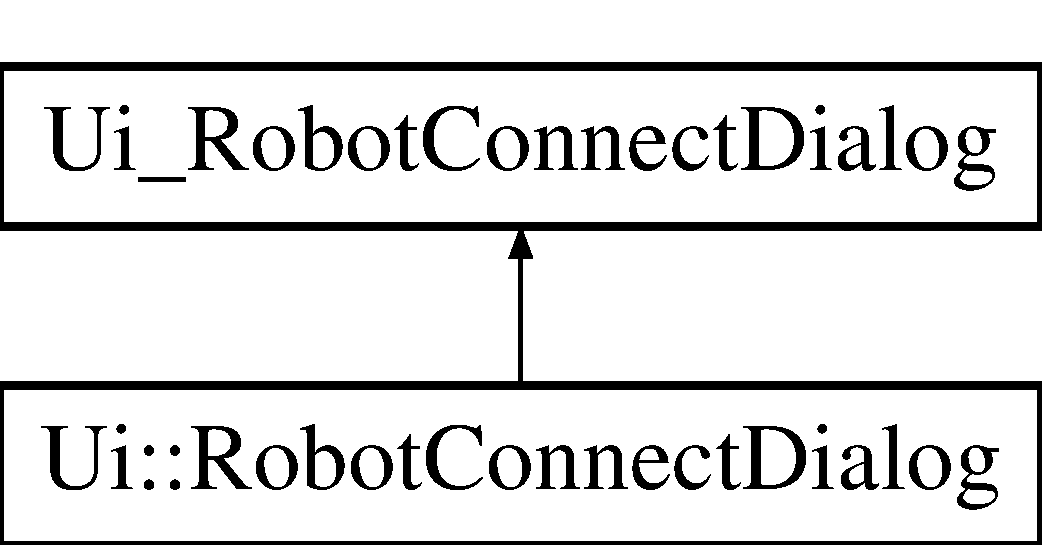
\includegraphics[height=2.000000cm]{classUi_1_1RobotConnectDialog}
\end{center}
\end{figure}
\subsection*{Additional Inherited Members}


The documentation for this class was generated from the following file\+:\begin{DoxyCompactItemize}
\item 
qt/\+Robot\+Station/build/ui\+\_\+robotconnectdialog.\+h\end{DoxyCompactItemize}

\hypertarget{classRobotConnectDialog}{}\section{Robot\+Connect\+Dialog Class Reference}
\label{classRobotConnectDialog}\index{Robot\+Connect\+Dialog@{Robot\+Connect\+Dialog}}
Inheritance diagram for Robot\+Connect\+Dialog\+:\begin{figure}[H]
\begin{center}
\leavevmode
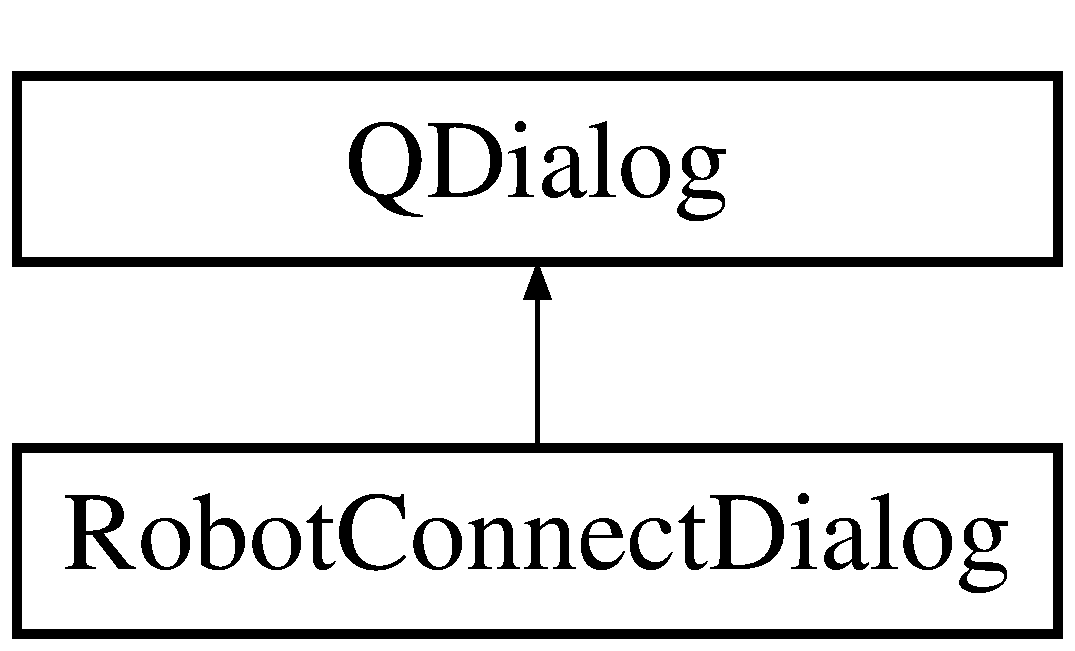
\includegraphics[height=2.000000cm]{classRobotConnectDialog}
\end{center}
\end{figure}
\subsection*{Public Member Functions}
\begin{DoxyCompactItemize}
\item 
\hypertarget{classRobotConnectDialog_afc50098da2f50179bb5f39c68c39efaa}{}{\bfseries Robot\+Connect\+Dialog} (Q\+Widget $\ast$parent=0)\label{classRobotConnectDialog_afc50098da2f50179bb5f39c68c39efaa}

\item 
\hypertarget{classRobotConnectDialog_ae70640758f8facacf04d0e3dec9ba3ed}{}std\+::string {\bfseries get\+I\+P\+Address} ()\label{classRobotConnectDialog_ae70640758f8facacf04d0e3dec9ba3ed}

\item 
\hypertarget{classRobotConnectDialog_a4ba40c51051147b3049248293ab6c744}{}std\+::string {\bfseries get\+Port} ()\label{classRobotConnectDialog_a4ba40c51051147b3049248293ab6c744}

\end{DoxyCompactItemize}


The documentation for this class was generated from the following files\+:\begin{DoxyCompactItemize}
\item 
qt/\+Robot\+Station/robotconnectdialog.\+h\item 
qt/\+Robot\+Station/robotconnectdialog.\+cpp\end{DoxyCompactItemize}

\hypertarget{classrbp_1_1Sensor}{}\section{rbp\+:\+:Sensor Class Reference}
\label{classrbp_1_1Sensor}\index{rbp\+::\+Sensor@{rbp\+::\+Sensor}}


An abstract class for devices that can interface with the world.  




{\ttfamily \#include $<$Sensor.\+h$>$}

Inheritance diagram for rbp\+:\+:Sensor\+:\begin{figure}[H]
\begin{center}
\leavevmode
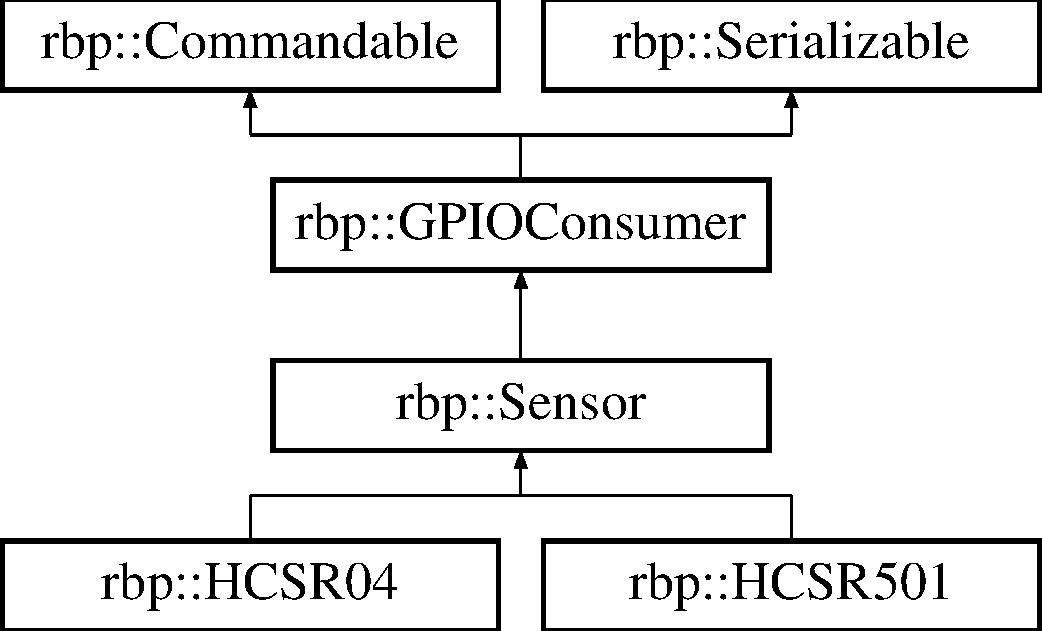
\includegraphics[height=4.000000cm]{classrbp_1_1Sensor}
\end{center}
\end{figure}
\subsection*{Public Member Functions}
\begin{DoxyCompactItemize}
\item 
virtual void \hyperlink{classrbp_1_1Sensor_ab9d45316bf67d871fddc7aa048e89c49}{Sense} ()=0
\begin{DoxyCompactList}\small\item\em Performs the sensor\textquotesingle{}s sensing operation. \end{DoxyCompactList}\end{DoxyCompactItemize}
\subsection*{Protected Member Functions}
\begin{DoxyCompactItemize}
\item 
void \hyperlink{classrbp_1_1Sensor_aab6baaef855fd31dab94e5b28386410a}{Set\+Output\+Pin} (int pin)
\begin{DoxyCompactList}\small\item\em Set an output pin for the sensor. \end{DoxyCompactList}\item 
void \hyperlink{classrbp_1_1Sensor_a2e3a00de93b77ecf39b4bfee79279c3c}{Set\+Input\+Pin} (int pin)
\begin{DoxyCompactList}\small\item\em Set an input pin for the sensor. \end{DoxyCompactList}\end{DoxyCompactItemize}


\subsection{Detailed Description}
An abstract class for devices that can interface with the world. 

Sensors can sense the world and provide valuable data about the state of the current environment.

Most sensors require an output, or a trigger, G\+P\+I\+O pin that tells the sensor when to sense. An example of this type of sensor is the \hyperlink{classrbp_1_1HCSR04}{H\+C\+S\+R04} ultrasonic distance sensor. However, there are sensors that persistently report its value back to a G\+P\+I\+O pin. An example of this type of sensor is the \hyperlink{classrbp_1_1HCSR501}{H\+C\+S\+R501} passive infrared sensor.

In both cases, there is a need for either an output pin and/or an input pin. 

\subsection{Member Function Documentation}
\hypertarget{classrbp_1_1Sensor_ab9d45316bf67d871fddc7aa048e89c49}{}\index{rbp\+::\+Sensor@{rbp\+::\+Sensor}!Sense@{Sense}}
\index{Sense@{Sense}!rbp\+::\+Sensor@{rbp\+::\+Sensor}}
\subsubsection[{Sense}]{\setlength{\rightskip}{0pt plus 5cm}virtual void rbp\+::\+Sensor\+::\+Sense (
\begin{DoxyParamCaption}
{}
\end{DoxyParamCaption}
)\hspace{0.3cm}{\ttfamily [pure virtual]}}\label{classrbp_1_1Sensor_ab9d45316bf67d871fddc7aa048e89c49}


Performs the sensor\textquotesingle{}s sensing operation. 

This method will retrieve a value from the environment by performing G\+P\+I\+O operations on the input and output pins of the sensor. The value from the sensor will be available through an accessor method. 

Implemented in \hyperlink{classrbp_1_1HCSR04_a8f8cc45655cacfb94ade5078c40ab1ba}{rbp\+::\+H\+C\+S\+R04}, and \hyperlink{classrbp_1_1HCSR501_a9b0e9b6f210d269b67a1ec94e3b62359}{rbp\+::\+H\+C\+S\+R501}.

\hypertarget{classrbp_1_1Sensor_a2e3a00de93b77ecf39b4bfee79279c3c}{}\index{rbp\+::\+Sensor@{rbp\+::\+Sensor}!Set\+Input\+Pin@{Set\+Input\+Pin}}
\index{Set\+Input\+Pin@{Set\+Input\+Pin}!rbp\+::\+Sensor@{rbp\+::\+Sensor}}
\subsubsection[{Set\+Input\+Pin}]{\setlength{\rightskip}{0pt plus 5cm}void rbp\+::\+Sensor\+::\+Set\+Input\+Pin (
\begin{DoxyParamCaption}
\item[{int}]{pin}
\end{DoxyParamCaption}
)\hspace{0.3cm}{\ttfamily [protected]}}\label{classrbp_1_1Sensor_a2e3a00de93b77ecf39b4bfee79279c3c}


Set an input pin for the sensor. 

Consumes a pin to be designated as an input. This is usually the pin that will be receiving data from the sensor.


\begin{DoxyParams}{Parameters}
{\em Pin} & The pin to designate as in input \\
\hline
\end{DoxyParams}
\hypertarget{classrbp_1_1Sensor_aab6baaef855fd31dab94e5b28386410a}{}\index{rbp\+::\+Sensor@{rbp\+::\+Sensor}!Set\+Output\+Pin@{Set\+Output\+Pin}}
\index{Set\+Output\+Pin@{Set\+Output\+Pin}!rbp\+::\+Sensor@{rbp\+::\+Sensor}}
\subsubsection[{Set\+Output\+Pin}]{\setlength{\rightskip}{0pt plus 5cm}void rbp\+::\+Sensor\+::\+Set\+Output\+Pin (
\begin{DoxyParamCaption}
\item[{int}]{pin}
\end{DoxyParamCaption}
)\hspace{0.3cm}{\ttfamily [protected]}}\label{classrbp_1_1Sensor_aab6baaef855fd31dab94e5b28386410a}


Set an output pin for the sensor. 

Consumes a pin to be designated as an output. This is usually the pin that triggers sensing.


\begin{DoxyParams}{Parameters}
{\em Pin} & The pin to designate as an output \\
\hline
\end{DoxyParams}


The documentation for this class was generated from the following files\+:\begin{DoxyCompactItemize}
\item 
include/raspboop/abstracts/Sensor.\+h\item 
src/abstracts/Sensor.\+cpp\end{DoxyCompactItemize}

\hypertarget{classrbp_1_1Serializable}{}\section{rbp\+:\+:Serializable Class Reference}
\label{classrbp_1_1Serializable}\index{rbp\+::\+Serializable@{rbp\+::\+Serializable}}


Interface for objects that can be serialized.  




{\ttfamily \#include $<$Serializable.\+h$>$}

Inheritance diagram for rbp\+:\+:Serializable\+:\begin{figure}[H]
\begin{center}
\leavevmode
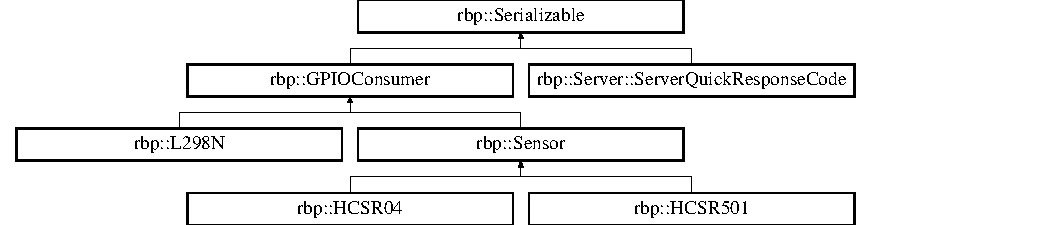
\includegraphics[height=3.022942cm]{classrbp_1_1Serializable}
\end{center}
\end{figure}
\subsection*{Public Member Functions}
\begin{DoxyCompactItemize}
\item 
virtual std\+::vector$<$ unsigned char $>$ \hyperlink{classrbp_1_1Serializable_a349896f5c3356330f914621033fda0bb}{Serialize} ()=0
\begin{DoxyCompactList}\small\item\em Returns an array representation of an object. \end{DoxyCompactList}\end{DoxyCompactItemize}


\subsection{Detailed Description}
Interface for objects that can be serialized. 



\subsection{Member Function Documentation}
\hypertarget{classrbp_1_1Serializable_a349896f5c3356330f914621033fda0bb}{}\index{rbp\+::\+Serializable@{rbp\+::\+Serializable}!Serialize@{Serialize}}
\index{Serialize@{Serialize}!rbp\+::\+Serializable@{rbp\+::\+Serializable}}
\subsubsection[{Serialize}]{\setlength{\rightskip}{0pt plus 5cm}virtual std\+::vector$<$unsigned char$>$ rbp\+::\+Serializable\+::\+Serialize (
\begin{DoxyParamCaption}
{}
\end{DoxyParamCaption}
)\hspace{0.3cm}{\ttfamily [pure virtual]}}\label{classrbp_1_1Serializable_a349896f5c3356330f914621033fda0bb}


Returns an array representation of an object. 

\begin{DoxyReturn}{Returns}
The Buffer of data 
\end{DoxyReturn}


Implemented in \hyperlink{classrbp_1_1L298N_a9f05ae8fd5d1d15584f4afe4f59e0f1f}{rbp\+::\+L298\+N}, \hyperlink{classrbp_1_1HCSR04_aa4a535b88dfdf50a75a2374193038c32}{rbp\+::\+H\+C\+S\+R04}, \hyperlink{classrbp_1_1HCSR501_a6aa46721ed0dcba774435a24ac17072e}{rbp\+::\+H\+C\+S\+R501}, and \hyperlink{classrbp_1_1Server_1_1ServerQuickResponseCode_a1b1aad62ce4446ec6aeb203ea67e9833}{rbp\+::\+Server\+::\+Server\+Quick\+Response\+Code}.



The documentation for this class was generated from the following file\+:\begin{DoxyCompactItemize}
\item 
include/raspboop/interfaces/Serializable.\+h\end{DoxyCompactItemize}

\hypertarget{classrbp_1_1Server}{}\section{rbp\+:\+:Server Class Reference}
\label{classrbp_1_1Server}\index{rbp\+::\+Server@{rbp\+::\+Server}}


\hyperlink{classrbp_1_1Server}{Server} class used to receive Commands.  




{\ttfamily \#include $<$Server.\+h$>$}

\subsection*{Classes}
\begin{DoxyCompactItemize}
\item 
class \hyperlink{classrbp_1_1Server_1_1ServerQuickResponseCode}{Server\+Quick\+Response\+Code}
\begin{DoxyCompactList}\small\item\em A convenience class used to quickly send a response code. \end{DoxyCompactList}\end{DoxyCompactItemize}
\subsection*{Public Types}
\begin{DoxyCompactItemize}
\item 
\hypertarget{classrbp_1_1Server_a8119bb8694bfa5cc978c38373ab23852}{}typedef std\+::function$<$ void(const \hyperlink{classrbp_1_1Command}{Command} $\ast$, \hyperlink{classrbp_1_1Server}{Server} $\ast$)$>$ {\bfseries Server\+Callback}\label{classrbp_1_1Server_a8119bb8694bfa5cc978c38373ab23852}

\end{DoxyCompactItemize}
\subsection*{Public Member Functions}
\begin{DoxyCompactItemize}
\item 
\hyperlink{classrbp_1_1Server_aeabc2e895aeae85e9d34acc6c3b2bc8f}{Server} (int port=9034)
\begin{DoxyCompactList}\small\item\em Instantiates a \hyperlink{classrbp_1_1Server}{Server} with a specified port. \end{DoxyCompactList}\item 
void \hyperlink{classrbp_1_1Server_a37deb0bbb0098f2148e7c21d6764c79a}{Add\+Callback} (Server\+Callback callback)
\begin{DoxyCompactList}\small\item\em Add a callback which will be invokes when a new, valid \hyperlink{classrbp_1_1Command}{Command} is received. \end{DoxyCompactList}\item 
void \hyperlink{classrbp_1_1Server_aab0491afac0864f0677766101b069778}{Enable\+Autodiscovery} (std\+::string interface, std\+::string group=\char`\"{}239.\+255.\+101.\+33\char`\"{}, int port=30001)
\begin{DoxyCompactList}\small\item\em Begins multicasting the \hyperlink{classrbp_1_1Server}{Server}\textquotesingle{}s I\+P and port. \end{DoxyCompactList}\item 
\hypertarget{classrbp_1_1Server_a64d00e53482b431692144df3fdc2b445}{}void \hyperlink{classrbp_1_1Server_a64d00e53482b431692144df3fdc2b445}{Start} ()\label{classrbp_1_1Server_a64d00e53482b431692144df3fdc2b445}

\begin{DoxyCompactList}\small\item\em Starts receiving data and begins multicasting if enabled. \end{DoxyCompactList}\item 
void \hyperlink{classrbp_1_1Server_a250e72cfa217fb8d6a31593f0eca6276}{Send\+Data} (\hyperlink{classrbp_1_1Serializable}{Serializable} $\ast$data)
\begin{DoxyCompactList}\small\item\em Sends a \hyperlink{classrbp_1_1Serializable}{Serializable} to the most recent client. \end{DoxyCompactList}\item 
\hypertarget{classrbp_1_1Server_a6a085077d0b2f48443428aa01e753798}{}void \hyperlink{classrbp_1_1Server_a6a085077d0b2f48443428aa01e753798}{Stop} ()\label{classrbp_1_1Server_a6a085077d0b2f48443428aa01e753798}

\begin{DoxyCompactList}\small\item\em Stops receiving data and stops multicasting if enabled. \end{DoxyCompactList}\end{DoxyCompactItemize}


\subsection{Detailed Description}
\hyperlink{classrbp_1_1Server}{Server} class used to receive Commands. 

The \hyperlink{classrbp_1_1Server}{Server} class uses U\+D\+P Sockets to exchange information as encoded and decoded by the \hyperlink{classrbp_1_1Command}{Command} class and the Raspboop Transmission Protocol.

The \hyperlink{classrbp_1_1Server}{Server} class also provides automatic discovery functionality through a Multicast sockets. Invoke \hyperlink{classrbp_1_1Server_aab0491afac0864f0677766101b069778}{Enable\+Autodiscovery()} to start Multicasting. 

\subsection{Constructor \& Destructor Documentation}
\hypertarget{classrbp_1_1Server_aeabc2e895aeae85e9d34acc6c3b2bc8f}{}\index{rbp\+::\+Server@{rbp\+::\+Server}!Server@{Server}}
\index{Server@{Server}!rbp\+::\+Server@{rbp\+::\+Server}}
\subsubsection[{Server}]{\setlength{\rightskip}{0pt plus 5cm}rbp\+::\+Server\+::\+Server (
\begin{DoxyParamCaption}
\item[{int}]{port = {\ttfamily 9034}}
\end{DoxyParamCaption}
)}\label{classrbp_1_1Server_aeabc2e895aeae85e9d34acc6c3b2bc8f}


Instantiates a \hyperlink{classrbp_1_1Server}{Server} with a specified port. 


\begin{DoxyParams}{Parameters}
{\em port} & The port to bind to. Default is 9034 \\
\hline
\end{DoxyParams}


\subsection{Member Function Documentation}
\hypertarget{classrbp_1_1Server_a37deb0bbb0098f2148e7c21d6764c79a}{}\index{rbp\+::\+Server@{rbp\+::\+Server}!Add\+Callback@{Add\+Callback}}
\index{Add\+Callback@{Add\+Callback}!rbp\+::\+Server@{rbp\+::\+Server}}
\subsubsection[{Add\+Callback}]{\setlength{\rightskip}{0pt plus 5cm}void rbp\+::\+Server\+::\+Add\+Callback (
\begin{DoxyParamCaption}
\item[{Server\+Callback}]{callback}
\end{DoxyParamCaption}
)}\label{classrbp_1_1Server_a37deb0bbb0098f2148e7c21d6764c79a}


Add a callback which will be invokes when a new, valid \hyperlink{classrbp_1_1Command}{Command} is received. 


\begin{DoxyParams}{Parameters}
{\em callback} & The callback to add \\
\hline
\end{DoxyParams}
\hypertarget{classrbp_1_1Server_aab0491afac0864f0677766101b069778}{}\index{rbp\+::\+Server@{rbp\+::\+Server}!Enable\+Autodiscovery@{Enable\+Autodiscovery}}
\index{Enable\+Autodiscovery@{Enable\+Autodiscovery}!rbp\+::\+Server@{rbp\+::\+Server}}
\subsubsection[{Enable\+Autodiscovery}]{\setlength{\rightskip}{0pt plus 5cm}void rbp\+::\+Server\+::\+Enable\+Autodiscovery (
\begin{DoxyParamCaption}
\item[{std\+::string}]{interface, }
\item[{std\+::string}]{group = {\ttfamily \char`\"{}239.255.101.33\char`\"{}}, }
\item[{int}]{port = {\ttfamily 30001}}
\end{DoxyParamCaption}
)}\label{classrbp_1_1Server_aab0491afac0864f0677766101b069778}


Begins multicasting the \hyperlink{classrbp_1_1Server}{Server}\textquotesingle{}s I\+P and port. 


\begin{DoxyParams}{Parameters}
{\em interface} & The I\+P of the machine on which the server is running \\
\hline
{\em group} & The I\+P of the multicast group. Default is 239.\+255.\+101.\+33 \\
\hline
{\em port} & The port of the multicast group. Default is 30001 \\
\hline
\end{DoxyParams}
\hypertarget{classrbp_1_1Server_a250e72cfa217fb8d6a31593f0eca6276}{}\index{rbp\+::\+Server@{rbp\+::\+Server}!Send\+Data@{Send\+Data}}
\index{Send\+Data@{Send\+Data}!rbp\+::\+Server@{rbp\+::\+Server}}
\subsubsection[{Send\+Data}]{\setlength{\rightskip}{0pt plus 5cm}void rbp\+::\+Server\+::\+Send\+Data (
\begin{DoxyParamCaption}
\item[{{\bf Serializable} $\ast$}]{data}
\end{DoxyParamCaption}
)}\label{classrbp_1_1Server_a250e72cfa217fb8d6a31593f0eca6276}


Sends a \hyperlink{classrbp_1_1Serializable}{Serializable} to the most recent client. 


\begin{DoxyParams}{Parameters}
{\em data} & The \hyperlink{classrbp_1_1Serializable}{Serializable} to send \\
\hline
\end{DoxyParams}


The documentation for this class was generated from the following files\+:\begin{DoxyCompactItemize}
\item 
include/raspboop/com/Server.\+h\item 
src/com/Server.\+cpp\end{DoxyCompactItemize}

\hypertarget{classrbp_1_1Server_1_1ServerQuickResponseCode}{}\section{rbp\+:\+:Server\+:\+:Server\+Quick\+Response\+Code Class Reference}
\label{classrbp_1_1Server_1_1ServerQuickResponseCode}\index{rbp\+::\+Server\+::\+Server\+Quick\+Response\+Code@{rbp\+::\+Server\+::\+Server\+Quick\+Response\+Code}}


A convenience class used to quickly send a response code.  




{\ttfamily \#include $<$Server.\+h$>$}

Inheritance diagram for rbp\+:\+:Server\+:\+:Server\+Quick\+Response\+Code\+:\begin{figure}[H]
\begin{center}
\leavevmode
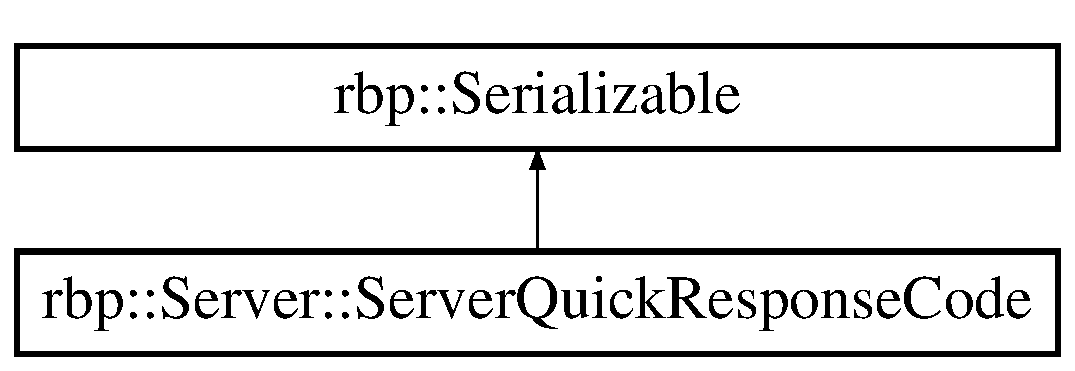
\includegraphics[height=2.000000cm]{classrbp_1_1Server_1_1ServerQuickResponseCode}
\end{center}
\end{figure}
\subsection*{Public Member Functions}
\begin{DoxyCompactItemize}
\item 
\hypertarget{classrbp_1_1Server_1_1ServerQuickResponseCode_a9b45a7422f3fff0c0d3132374151ae85}{}{\bfseries Server\+Quick\+Response\+Code} (unsigned char response\+Code)\label{classrbp_1_1Server_1_1ServerQuickResponseCode_a9b45a7422f3fff0c0d3132374151ae85}

\item 
virtual std\+::vector$<$ unsigned char $>$ \hyperlink{classrbp_1_1Server_1_1ServerQuickResponseCode_a1b1aad62ce4446ec6aeb203ea67e9833}{Serialize} ()
\begin{DoxyCompactList}\small\item\em Returns an array representation of an object. \end{DoxyCompactList}\end{DoxyCompactItemize}
\subsection*{Public Attributes}
\begin{DoxyCompactItemize}
\item 
\hypertarget{classrbp_1_1Server_1_1ServerQuickResponseCode_af1d520d92e825fdb59d7a225e706ca38}{}unsigned char {\bfseries m\+Response\+Code}\label{classrbp_1_1Server_1_1ServerQuickResponseCode_af1d520d92e825fdb59d7a225e706ca38}

\end{DoxyCompactItemize}


\subsection{Detailed Description}
A convenience class used to quickly send a response code. 

\subsection{Member Function Documentation}
\hypertarget{classrbp_1_1Server_1_1ServerQuickResponseCode_a1b1aad62ce4446ec6aeb203ea67e9833}{}\index{rbp\+::\+Server\+::\+Server\+Quick\+Response\+Code@{rbp\+::\+Server\+::\+Server\+Quick\+Response\+Code}!Serialize@{Serialize}}
\index{Serialize@{Serialize}!rbp\+::\+Server\+::\+Server\+Quick\+Response\+Code@{rbp\+::\+Server\+::\+Server\+Quick\+Response\+Code}}
\subsubsection[{Serialize}]{\setlength{\rightskip}{0pt plus 5cm}virtual std\+::vector$<$unsigned char$>$ rbp\+::\+Server\+::\+Server\+Quick\+Response\+Code\+::\+Serialize (
\begin{DoxyParamCaption}
{}
\end{DoxyParamCaption}
)\hspace{0.3cm}{\ttfamily [inline]}, {\ttfamily [virtual]}}\label{classrbp_1_1Server_1_1ServerQuickResponseCode_a1b1aad62ce4446ec6aeb203ea67e9833}


Returns an array representation of an object. 

\begin{DoxyReturn}{Returns}
The Buffer of data 
\end{DoxyReturn}


Implements \hyperlink{classrbp_1_1Serializable_a349896f5c3356330f914621033fda0bb}{rbp\+::\+Serializable}.



The documentation for this class was generated from the following file\+:\begin{DoxyCompactItemize}
\item 
include/raspboop/com/Server.\+h\end{DoxyCompactItemize}

\hypertarget{classStationWindow}{}\section{Station\+Window Class Reference}
\label{classStationWindow}\index{Station\+Window@{Station\+Window}}
Inheritance diagram for Station\+Window\+:\begin{figure}[H]
\begin{center}
\leavevmode
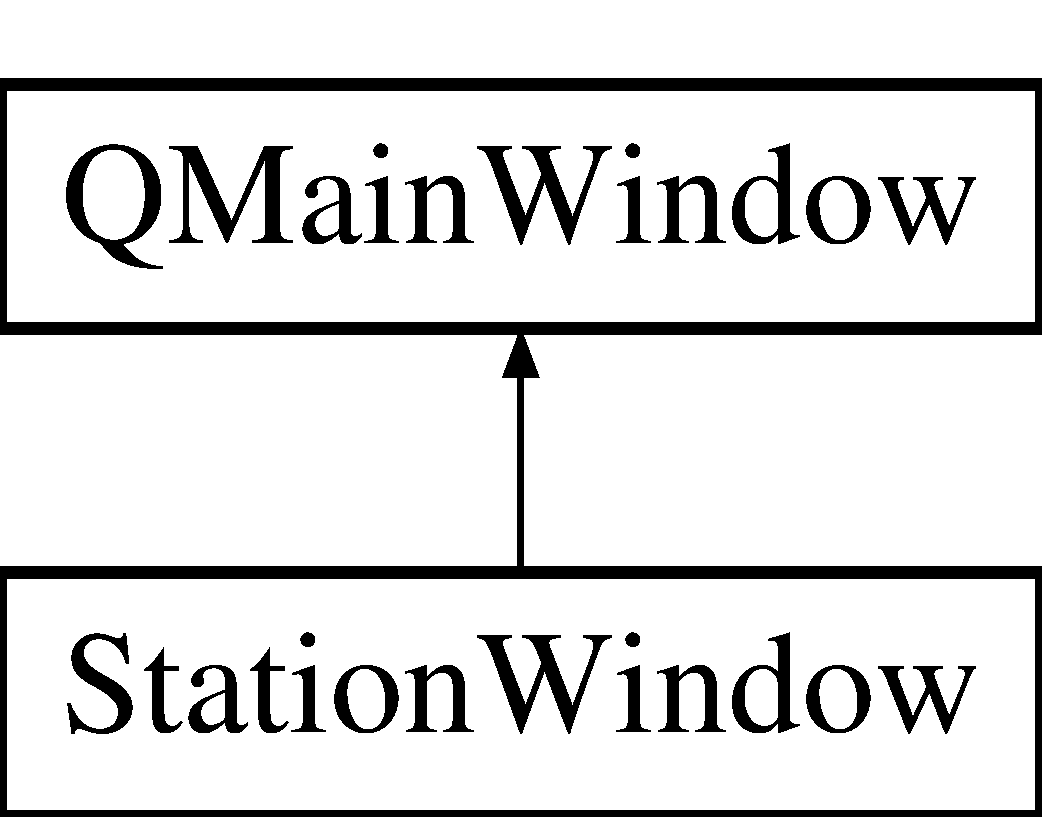
\includegraphics[height=2.000000cm]{classStationWindow}
\end{center}
\end{figure}
\subsection*{Public Member Functions}
\begin{DoxyCompactItemize}
\item 
\hypertarget{classStationWindow_a0458e1bdc1b8feb165180ff7e30dfac4}{}{\bfseries Station\+Window} (Q\+Widget $\ast$parent=0)\label{classStationWindow_a0458e1bdc1b8feb165180ff7e30dfac4}

\end{DoxyCompactItemize}


The documentation for this class was generated from the following files\+:\begin{DoxyCompactItemize}
\item 
qt/\+Robot\+Station/stationwindow.\+h\item 
qt/\+Robot\+Station/stationwindow.\+cpp\end{DoxyCompactItemize}

\hypertarget{classUi_1_1StationWindow}{}\section{Ui\+:\+:Station\+Window Class Reference}
\label{classUi_1_1StationWindow}\index{Ui\+::\+Station\+Window@{Ui\+::\+Station\+Window}}
Inheritance diagram for Ui\+:\+:Station\+Window\+:\begin{figure}[H]
\begin{center}
\leavevmode
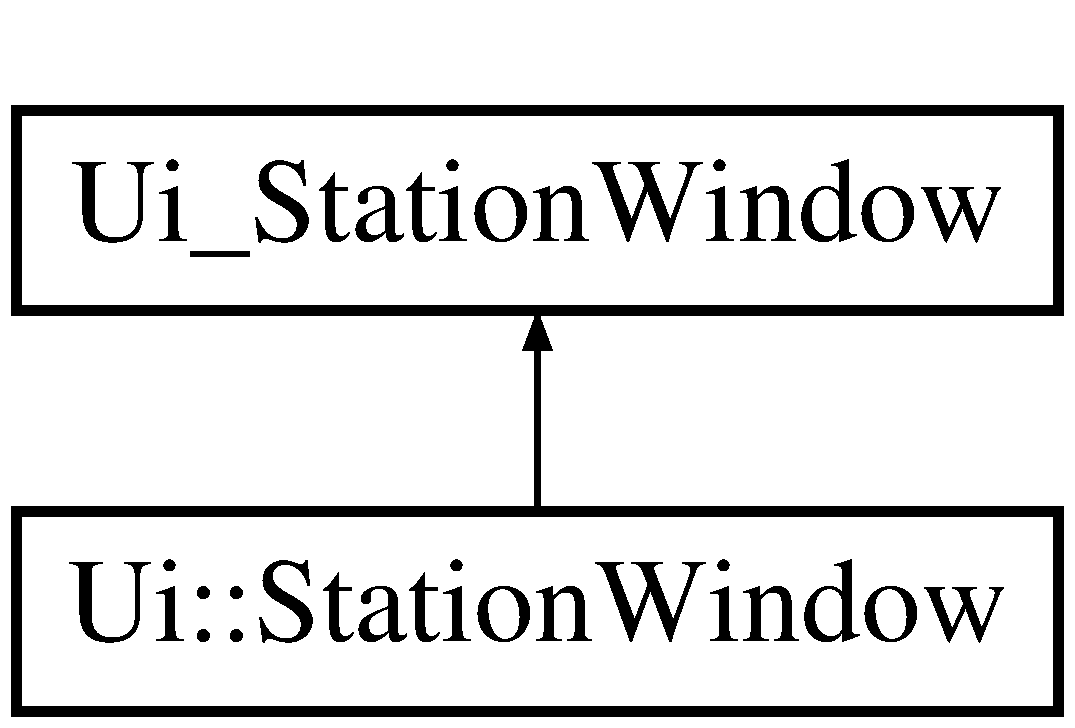
\includegraphics[height=2.000000cm]{classUi_1_1StationWindow}
\end{center}
\end{figure}
\subsection*{Additional Inherited Members}


The documentation for this class was generated from the following file\+:\begin{DoxyCompactItemize}
\item 
qt/\+Robot\+Station/build/ui\+\_\+stationwindow.\+h\end{DoxyCompactItemize}

\hypertarget{classUi__RobotConnectDialog}{}\section{Ui\+\_\+\+Robot\+Connect\+Dialog Class Reference}
\label{classUi__RobotConnectDialog}\index{Ui\+\_\+\+Robot\+Connect\+Dialog@{Ui\+\_\+\+Robot\+Connect\+Dialog}}
Inheritance diagram for Ui\+\_\+\+Robot\+Connect\+Dialog\+:\begin{figure}[H]
\begin{center}
\leavevmode
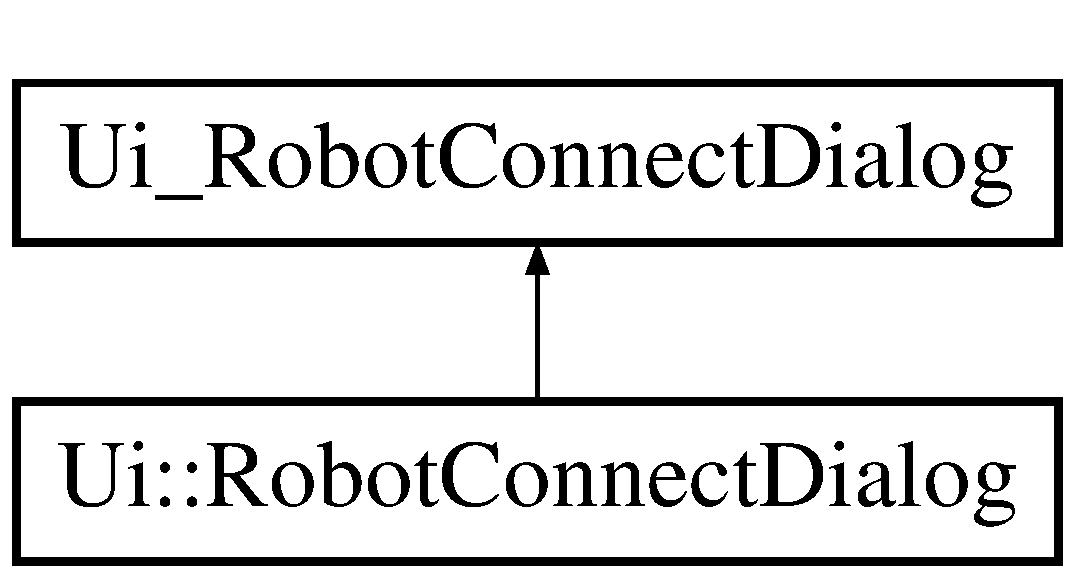
\includegraphics[height=2.000000cm]{classUi__RobotConnectDialog}
\end{center}
\end{figure}
\subsection*{Public Member Functions}
\begin{DoxyCompactItemize}
\item 
\hypertarget{classUi__RobotConnectDialog_a78d76df0eddc0a7ab4efa825cca8bb2f}{}void {\bfseries setup\+Ui} (Q\+Dialog $\ast$\hyperlink{classRobotConnectDialog}{Robot\+Connect\+Dialog})\label{classUi__RobotConnectDialog_a78d76df0eddc0a7ab4efa825cca8bb2f}

\item 
\hypertarget{classUi__RobotConnectDialog_ae9b4da508c51dcd0992ba2c3624448c0}{}void {\bfseries retranslate\+Ui} (Q\+Dialog $\ast$\hyperlink{classRobotConnectDialog}{Robot\+Connect\+Dialog})\label{classUi__RobotConnectDialog_ae9b4da508c51dcd0992ba2c3624448c0}

\end{DoxyCompactItemize}
\subsection*{Public Attributes}
\begin{DoxyCompactItemize}
\item 
\hypertarget{classUi__RobotConnectDialog_a58446348e7f5a038f0f813a8945718e4}{}Q\+V\+Box\+Layout $\ast$ {\bfseries vertical\+Layout}\label{classUi__RobotConnectDialog_a58446348e7f5a038f0f813a8945718e4}

\item 
\hypertarget{classUi__RobotConnectDialog_afdc5c4c69c6925f72f928d12649d918b}{}Q\+Tab\+Widget $\ast$ {\bfseries tab\+Widget}\label{classUi__RobotConnectDialog_afdc5c4c69c6925f72f928d12649d918b}

\item 
\hypertarget{classUi__RobotConnectDialog_a92054520d0c79a83cafbde9eba32159e}{}Q\+Widget $\ast$ {\bfseries ip\+\_\+tab}\label{classUi__RobotConnectDialog_a92054520d0c79a83cafbde9eba32159e}

\item 
\hypertarget{classUi__RobotConnectDialog_a4ddd5c41f38ba72340b26ee45c64813f}{}Q\+V\+Box\+Layout $\ast$ {\bfseries vertical\+Layout\+\_\+2}\label{classUi__RobotConnectDialog_a4ddd5c41f38ba72340b26ee45c64813f}

\item 
\hypertarget{classUi__RobotConnectDialog_ac41a39c9ebaba85b81cc6192ac68314f}{}Q\+Form\+Layout $\ast$ {\bfseries form\+Layout}\label{classUi__RobotConnectDialog_ac41a39c9ebaba85b81cc6192ac68314f}

\item 
\hypertarget{classUi__RobotConnectDialog_ae47b7d2cdbc5338b43f1d664cb29562e}{}Q\+Label $\ast$ {\bfseries label}\label{classUi__RobotConnectDialog_ae47b7d2cdbc5338b43f1d664cb29562e}

\item 
\hypertarget{classUi__RobotConnectDialog_a02fdb9586a566fdc5b337d281f56b8c6}{}Q\+Line\+Edit $\ast$ {\bfseries line\+Edit}\label{classUi__RobotConnectDialog_a02fdb9586a566fdc5b337d281f56b8c6}

\item 
\hypertarget{classUi__RobotConnectDialog_a0c1c2d097116445ebd6de61926548873}{}Q\+Label $\ast$ {\bfseries label\+\_\+2}\label{classUi__RobotConnectDialog_a0c1c2d097116445ebd6de61926548873}

\item 
\hypertarget{classUi__RobotConnectDialog_af5a93ee9b5881e19ca4c1d33d381f4cd}{}Q\+Line\+Edit $\ast$ {\bfseries line\+Edit\+\_\+2}\label{classUi__RobotConnectDialog_af5a93ee9b5881e19ca4c1d33d381f4cd}

\item 
\hypertarget{classUi__RobotConnectDialog_a785d5f08f5aaa596ad50cf3e2e9dd2bb}{}Q\+Spacer\+Item $\ast$ {\bfseries vertical\+Spacer}\label{classUi__RobotConnectDialog_a785d5f08f5aaa596ad50cf3e2e9dd2bb}

\item 
\hypertarget{classUi__RobotConnectDialog_a6342c327401d66f955c081c61817137a}{}Q\+H\+Box\+Layout $\ast$ {\bfseries horizontal\+Layout}\label{classUi__RobotConnectDialog_a6342c327401d66f955c081c61817137a}

\item 
\hypertarget{classUi__RobotConnectDialog_a905b9b5570a38625704fcbd9d1965160}{}Q\+Spacer\+Item $\ast$ {\bfseries horizontal\+Spacer}\label{classUi__RobotConnectDialog_a905b9b5570a38625704fcbd9d1965160}

\item 
\hypertarget{classUi__RobotConnectDialog_a4e95d3d3a674dacbbf0bb1d32a0d1fd5}{}Q\+Push\+Button $\ast$ {\bfseries ip\+\_\+button}\label{classUi__RobotConnectDialog_a4e95d3d3a674dacbbf0bb1d32a0d1fd5}

\item 
\hypertarget{classUi__RobotConnectDialog_aadccf8e2748e1faf921dc44a7de47d32}{}Q\+Widget $\ast$ {\bfseries multicast\+\_\+tab}\label{classUi__RobotConnectDialog_aadccf8e2748e1faf921dc44a7de47d32}

\item 
\hypertarget{classUi__RobotConnectDialog_a5cadc9362ad4faeb26bc0ae8c7d38be0}{}Q\+V\+Box\+Layout $\ast$ {\bfseries vertical\+Layout\+\_\+3}\label{classUi__RobotConnectDialog_a5cadc9362ad4faeb26bc0ae8c7d38be0}

\item 
\hypertarget{classUi__RobotConnectDialog_abb33148cd10ae2082a6c61dae283da71}{}Q\+Label $\ast$ {\bfseries label\+\_\+3}\label{classUi__RobotConnectDialog_abb33148cd10ae2082a6c61dae283da71}

\item 
\hypertarget{classUi__RobotConnectDialog_afa03a323647133f82b7e3969e082f59d}{}Q\+List\+View $\ast$ {\bfseries list\+View}\label{classUi__RobotConnectDialog_afa03a323647133f82b7e3969e082f59d}

\item 
\hypertarget{classUi__RobotConnectDialog_ad0d261340d2070ae9001ca82620b146a}{}Q\+H\+Box\+Layout $\ast$ {\bfseries horizontal\+Layout\+\_\+2}\label{classUi__RobotConnectDialog_ad0d261340d2070ae9001ca82620b146a}

\item 
\hypertarget{classUi__RobotConnectDialog_afe90b2289121449cccc81dcd8d19ab89}{}Q\+Spacer\+Item $\ast$ {\bfseries horizontal\+Spacer\+\_\+2}\label{classUi__RobotConnectDialog_afe90b2289121449cccc81dcd8d19ab89}

\item 
\hypertarget{classUi__RobotConnectDialog_a3fb2a63daac3e59200a2889656b9af52}{}Q\+Push\+Button $\ast$ {\bfseries multicast\+\_\+button}\label{classUi__RobotConnectDialog_a3fb2a63daac3e59200a2889656b9af52}

\end{DoxyCompactItemize}


The documentation for this class was generated from the following file\+:\begin{DoxyCompactItemize}
\item 
qt/\+Robot\+Station/build/ui\+\_\+robotconnectdialog.\+h\end{DoxyCompactItemize}

\hypertarget{classUi__StationWindow}{}\section{Ui\+\_\+\+Station\+Window Class Reference}
\label{classUi__StationWindow}\index{Ui\+\_\+\+Station\+Window@{Ui\+\_\+\+Station\+Window}}
Inheritance diagram for Ui\+\_\+\+Station\+Window\+:\begin{figure}[H]
\begin{center}
\leavevmode
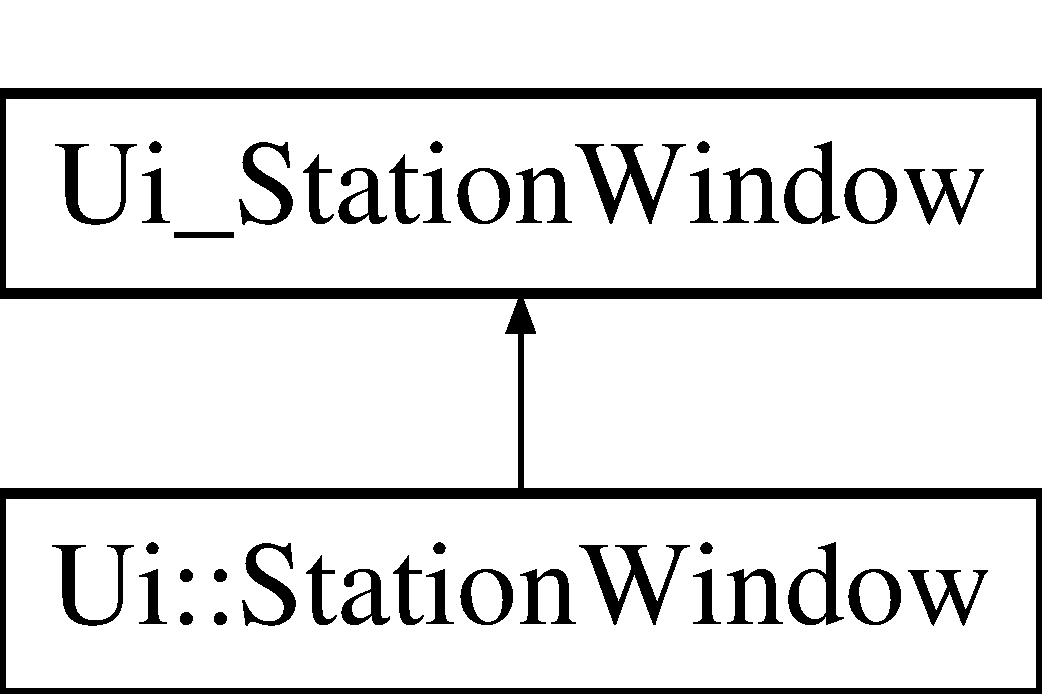
\includegraphics[height=2.000000cm]{classUi__StationWindow}
\end{center}
\end{figure}
\subsection*{Public Member Functions}
\begin{DoxyCompactItemize}
\item 
\hypertarget{classUi__StationWindow_ad46fc9769c9f4f37f99b87af82ea59a8}{}void {\bfseries setup\+Ui} (Q\+Main\+Window $\ast$\hyperlink{classStationWindow}{Station\+Window})\label{classUi__StationWindow_ad46fc9769c9f4f37f99b87af82ea59a8}

\item 
\hypertarget{classUi__StationWindow_aafe239252f157bcab7e3812258c4c4d3}{}void {\bfseries retranslate\+Ui} (Q\+Main\+Window $\ast$\hyperlink{classStationWindow}{Station\+Window})\label{classUi__StationWindow_aafe239252f157bcab7e3812258c4c4d3}

\end{DoxyCompactItemize}
\subsection*{Public Attributes}
\begin{DoxyCompactItemize}
\item 
\hypertarget{classUi__StationWindow_a29ad623f922ab7ede612f9dddab7a55c}{}Q\+Widget $\ast$ {\bfseries central\+Widget}\label{classUi__StationWindow_a29ad623f922ab7ede612f9dddab7a55c}

\item 
\hypertarget{classUi__StationWindow_a781611f8784156ed093f55133a25a8fe}{}Q\+Widget $\ast$ {\bfseries vertical\+Layout\+Widget}\label{classUi__StationWindow_a781611f8784156ed093f55133a25a8fe}

\item 
\hypertarget{classUi__StationWindow_a7993a098ec601f40393fcafd8cfa619e}{}Q\+V\+Box\+Layout $\ast$ {\bfseries vertical\+Layout}\label{classUi__StationWindow_a7993a098ec601f40393fcafd8cfa619e}

\item 
\hypertarget{classUi__StationWindow_ad015d1543bc1ca34a00d7a0972703fed}{}Q\+Push\+Button $\ast$ {\bfseries push\+Button}\label{classUi__StationWindow_ad015d1543bc1ca34a00d7a0972703fed}

\item 
\hypertarget{classUi__StationWindow_acd4d97d889710071df46b388cc41a59b}{}Q\+H\+Box\+Layout $\ast$ {\bfseries horizontal\+Layout}\label{classUi__StationWindow_acd4d97d889710071df46b388cc41a59b}

\item 
\hypertarget{classUi__StationWindow_a2c1e1c0a89df30ddceadcdbc336220e3}{}Q\+Label $\ast$ {\bfseries label}\label{classUi__StationWindow_a2c1e1c0a89df30ddceadcdbc336220e3}

\item 
\hypertarget{classUi__StationWindow_a69ba5662bd433c7ea4517e855f98ceef}{}Q\+Label $\ast$ {\bfseries label\+\_\+2}\label{classUi__StationWindow_a69ba5662bd433c7ea4517e855f98ceef}

\item 
\hypertarget{classUi__StationWindow_a26d848d23a49c55f53cb002c14bc4a6d}{}Q\+Frame $\ast$ {\bfseries frame}\label{classUi__StationWindow_a26d848d23a49c55f53cb002c14bc4a6d}

\item 
\hypertarget{classUi__StationWindow_a55e779c5080b58d5d184e62f940bebb5}{}Q\+Menu\+Bar $\ast$ {\bfseries menu\+Bar}\label{classUi__StationWindow_a55e779c5080b58d5d184e62f940bebb5}

\item 
\hypertarget{classUi__StationWindow_a42668dfd765d1f0530f5ea338a6777fd}{}Q\+Tool\+Bar $\ast$ {\bfseries main\+Tool\+Bar}\label{classUi__StationWindow_a42668dfd765d1f0530f5ea338a6777fd}

\item 
\hypertarget{classUi__StationWindow_afbc2e6b70ab385a9a163bfc80ef49299}{}Q\+Status\+Bar $\ast$ {\bfseries status\+Bar}\label{classUi__StationWindow_afbc2e6b70ab385a9a163bfc80ef49299}

\end{DoxyCompactItemize}


The documentation for this class was generated from the following file\+:\begin{DoxyCompactItemize}
\item 
qt/\+Robot\+Station/build/ui\+\_\+stationwindow.\+h\end{DoxyCompactItemize}

\hypertarget{classrbp_1_1WiringPiPins}{}\section{rbp\+:\+:Wiring\+Pi\+Pins Class Reference}
\label{classrbp_1_1WiringPiPins}\index{rbp\+::\+Wiring\+Pi\+Pins@{rbp\+::\+Wiring\+Pi\+Pins}}


A convenience class for the P1 G\+P\+I\+O Connector pins \href{http://wiringpi.com/pins/}{\tt Pin reference}  




{\ttfamily \#include $<$Types.\+h$>$}



\subsection{Detailed Description}
A convenience class for the P1 G\+P\+I\+O Connector pins \href{http://wiringpi.com/pins/}{\tt Pin reference} 

The documentation for this class was generated from the following file\+:\begin{DoxyCompactItemize}
\item 
include/raspboop/essentials/Types.\+h\end{DoxyCompactItemize}

\hypertarget{classrbp_1_1WiringPiPinsP5}{}\section{rbp\+:\+:Wiring\+Pi\+Pins\+P5 Class Reference}
\label{classrbp_1_1WiringPiPinsP5}\index{rbp\+::\+Wiring\+Pi\+Pins\+P5@{rbp\+::\+Wiring\+Pi\+Pins\+P5}}


A convenience class for the P5 connector on the Raspberry Pi Model B This class is specific to the Wiring\+Pi pin numbering \href{http://wiringpi.com/pins/}{\tt Pin reference}  




{\ttfamily \#include $<$Types.\+h$>$}



\subsection{Detailed Description}
A convenience class for the P5 connector on the Raspberry Pi Model B This class is specific to the Wiring\+Pi pin numbering \href{http://wiringpi.com/pins/}{\tt Pin reference} 

The documentation for this class was generated from the following file\+:\begin{DoxyCompactItemize}
\item 
include/raspboop/essentials/Types.\+h\end{DoxyCompactItemize}

%--- End generated contents ---

% Index
\backmatter
\newpage
\phantomsection
\clearemptydoublepage
\addcontentsline{toc}{chapter}{Index}
\printindex

\end{document}
